\documentclass[12pt, a4paper]{article}
\usepackage[dvipdfmx]{graphicx}
\usepackage{amssymb}
\usepackage{amsmath}
\usepackage{bm}
\usepackage{multirow}
\usepackage[table]{xcolor} %for \rowcolors
\usepackage{cite}
\usepackage{slashed}
\usepackage{subfigure}
\usepackage{epstopdf}            
\usepackage{epsfig}
\usepackage{here}
\usepackage{comment}
\usepackage{booktabs} %for \toprule
\usepackage{colortbl} %for \rowcolor
\usepackage{mathptmx} % change all font
\usepackage{wrapfig}
\usepackage{ascmac}
\usepackage{fancybox}  
\usepackage{ulem}
\usepackage{enumerate}
%\usepackage{mathpazo} % change all font
\DeclareMathAlphabet{\mathcal}{OMS}{cmsy}{m}{n} % change \mathcal 

\setlength\arraycolsep{2pt}

% -------------------------------------------------------- Page Styles
\setlength{\textwidth}{15.3cm}
\setlength{\textheight}{23.0cm}
\setlength{\oddsidemargin}{.3 cm}
\setlength{\evensidemargin}{0cm}
\setlength{\topmargin}{-.9cm}
\setlength{\footskip}{2.1cm}
% same as JHEP
\renewcommand{\thefootnote}{\fnsymbol{footnote}}
\numberwithin{equation}{section} % Eq.(Sec.eq.)


\renewcommand\citepunct{,\penalty1000\hskip.13emplus.1emminus.1em\relax} % no line-break in \cite
\def\beq#1\eeq{\begin{align}#1\end{align}}
\newcommand{\ov}{\overline}
\newcommand{\pa}{\partial}
\newcommand{\al}{\alpha}
\newcommand{\ep}{\epsilon}
\newcommand{\ka}{\kappa}

\newcommand{\Slash}[1]{{\ooalign{\hfil/\hfil\crcr$#1$}}}
\newcommand{\1}{\mbox{1}\hspace{-0.25em}\mbox{l}}

\renewcommand{\arraystretch}{1.3}

\newcommand{\pg}[1]{{\color{red}\bf #1}}
\newcommand{\pgc}[1]{{\color{red}\it (#1)}}
\newcommand{\ET}{\mbox{$\not \hspace{-0.10cm} E_T$ }}

\newcommand{\Kzerobar}{\overline{K}^0}
\newcommand{\Kstarzerobar}{\overline{K}^{\ts *0}}
\newcommand{\Dzerobar}{\overline{D}^0}
\newcommand{\Dstarzerobar}{\overline{D}^{\ts *0}}
\newcommand{\Bzerobar}{\overline{B}^0}
\newcommand{\Bsbar}{\overline{B}_s}
\newcommand{\IWxi}[1]{\xi^{(#1)}}
\newcommand{\IWet}[1]{\eta^{(#1)}}
\newcommand{\IWci}[2]{\hat\chi^{(#1)}_{#2}}
\newcommand{\IWel}[2]{\hat\ell^{(#1)}_{#2}}

\newcommand{\lv}{{L^\prime}}

% ----------------------------------------------------------- Meson
\RequirePackage{xspace}
\def\Bbar    {\kern 0.18em\overline{\kern -0.18em B}{}\xspace}
\def\Bb      {\ensuremath{\Bbar}\xspace}

% ----------------------------------------------------------- Caption
\usepackage{caption}
\captionsetup[figure]{format=plain,labelformat=simple,labelsep=period,font=small }
\captionsetup[table]{format=plain,labelformat=simple,labelsep=period,font=small }

% ----------------------------------------------------------- Hyperref
\definecolor{BlueViolet}{rgb}{0.2, 0.00, 0.7}
\definecolor{Blue}{rgb}{0.15, 0.00, 0.9}
\definecolor{light_blue}{rgb}{0.15, 0.35, 0.95}
\definecolor{kit_green}{rgb}{0, 
0.58823 %150/255
, 0.50980 %130/255
}
\usepackage[%dvipdfmx,
colorlinks=true, linkcolor=light_blue,citecolor=light_blue,urlcolor=kit_green]{hyperref} 

\newcommand{\si}[1]{\textcolor{blue}{#1}}
\newcommand{\yo}[1]{\textcolor{magenta}{#1}}
\renewcommand{\baselinestretch}{1.1} %space between the lines


\begin{document}
\sloppy %https://tex.stackexchange.com/questions/9107/how-can-i-make-my-text-never-go-over-the-right-margin-by-always-hyphenating-or-b

\begin{titlepage}
\begin{center}

\hfill{P3H--23--036, TTP23--20}
\vskip .3in
{\Large{\bf A closer look at isodoublet vector leptoquark\\ solution to the $R_{D^{(*)}}$ anomaly }}
\vskip .3in

% bold applies to math too
\makeatletter\g@addto@macro\bfseries{\boldmath}\makeatother

{\large 
Syuhei Iguro$^{\rm (a,b)}$,
Yuji Omura$^{\rm (c)}$
}
\vskip .3in

$^{\rm (a)}${\it Institute for Theoretical Particle Physics (TTP), Karlsruhe Institute of Technology (KIT),
Wolfgang-Gaede-Str.\,1, 76131 Karlsruhe, Germany}\\
\vspace{4.6pt}

$^{\rm (b)}${\it Institute for Astroparticle Physics (IAP),
Karlsruhe Institute of Technology (KIT), 
Hermann-von-Helmholtz-Platz 1, 76344 Eggenstein-Leopoldshafen, Germany}\\
\vspace{4.6pt}

$^{\rm (c)}${\it
Department of Physics, Kindai University, Higashi-Osaka, Osaka 577-8502, Japan}\\[3pt]

\> {\it E-mail:} \href{mailto:igurosyuhei@gmail.com}{igurosyuhei@gmail.com},
\href{mailto:yomura@phys.kindai.ac.jp}{yomura@phys.kindai.ac.jp},

\vskip 0.1in
%{Dated: January 24, 2023 (First)}\\
%{Dated: May 25, 2023 (Current update)}\\

\end{center}
\vskip .3in

%%%%%%%%%%%%%%%%%%%%%%%%%
\begin{abstract}


\noindent 
We discuss a model with a SU$(2)_L$ doublet vector leptoquark (LQ), motivated by 
the recent experimental results relating to the lepton universality of $\Bb \to D^{(*)} \tau \overline{\nu}_\tau$.
We find that scalar operators predicted by the LQ are favored to explain the deviations,
taking into account the recent LHCb result.
We investigate the extensive phenomenology of the model and conclude that $B_s\to\tau\ov\tau$, $B_u\to \tau\ov\nu_\tau$ and high-$p_T$ di-$\tau$ lepton signatures at the LHC will probe the interesting parameter region in the near future.

%%%%%%%%%%%%%%%%%%%%%%%%%
\end{abstract}
{\sc Keywords: Vector SU(2) doublet leptoquark, $R_{D^{(*)}}$ anomaly, LHC, flavor} 
%%%%%%%%%%%%%%%%%%%%%%%%%
\end{titlepage}

\setcounter{page}{1}
\renewcommand{\thefootnote}{\#\arabic{footnote}}
\setcounter{footnote}{0}

%%%%%%%%%%%%%%%%%%%%%%%%%
% Contents
%%%%%%%%%%%%%%%%%%%%%%%%%
\hrule
\tableofcontents
\vskip .2in
\hrule
\vskip .4in
%%%%%%%%%%%%%%%%%%%%%%%%%

%%%%%%%%%%%%%%%%%%%%%%%%%%%%%%%
\section{Introduction}
\label{sec:intro}
%%%%%%%%%%%%%%%%%%%%%%%%%%%%%%%
The semi-tauonic $B$-meson decays, $\Bb \to D^{(*)} \tau \ov\nu$, have been interesting processes to measure the lepton flavor universality (LFU):
 \begin{align}
  R_D \equiv \frac{{\rm{BR}}(\Bb\rightarrow D \,\tau\, \overline\nu_\tau)}{{\rm{BR}}(\Bb\rightarrow D\, \ell\,\overline\nu_\ell)} , \qquad
  R_{D^{*}} \equiv \frac{{\rm{BR}}(\Bb\rightarrow D^{*} \tau \,\overline\nu_\tau)}{{\rm{BR}}(\Bb\rightarrow D^{*} \ell\,\overline\nu_\ell)}, 
\end{align}
where $\ell$ denotes light charged leptons.
Interestingly, deviations from the SM predictions \cite{Bordone:2019guc,Iguro:2020cpg,HFLAV:2022pwe,Bernlochner:2022ywh}\footnote{Recently the dispersive matrix approach of the form factors found the larger $R_{D^*}$ \cite{Martinelli:2021onb,Martinelli:2021myh} based on the Fermilab-MILC lattice result \cite{FermilabLattice:2021cdg} while this method produce the $3\,\sigma$ tension in the angular observable \cite{Fedele:2023ewe}.} have been reported by 
the BaBar~\cite{Lees:2012xj,Lees:2013uzd}, Belle~\cite{Huschle:2015rga,Hirose:2016wfn,Hirose:2017dxl,Abdesselam:2019dgh,Belle:2019rba} and LHCb~\cite{Aaij:2015yra,Aaij:2017uff,Aaij:2017deq,LHCb:2023zxo,LHCbRun1had} collaborations.\footnote{$R_{D^{(*)}}$ are defined by $\ell =e,~\mu$ for the BaBar/Belle and $\ell =\mu$ for the LHCb.}
Last and early this years, the LHCb collaboration reported the first result of $R_{D^*}$ along with $R_{D}$ \cite{Ciezarek:2837207} and another $R_{D^*}$ data \cite{LHCbRDst2023}, respectively.
These latest measurements are consistent with the previous world average within the uncertainty, but the resulting world average prefers larger (smaller) deviation in $R_{D}$ ($R_{D^*}$).
The current significance of the deviation is 3-4\,$\sigma$ \cite{Iguro:2022yzr} and the new physics (NP) interpretations are updated in Refs.\,\cite{Iguro:2022yzr,Aebischer:2022oqe,Fedele:2022iib,Aban:2023pgq}.\footnote{See Tab.\,6 of Ref.\,\cite{Iguro:2022yzr} for the recent summary of the situation.}
One of the significant points, compared with the previous result, is the revival of the NP interpretation with scalar operators.
The relevant interaction, in addition to the SM contribution, is
\begin{align}
 {\cal {H}}_{\rm{eff}}= 2 \sqrt2 G_FV_{cb}\biggl[ C_{S_L}O_{S_L}+C_{S_
R}O_{S_R}\biggl],
\label{eq:Ham_bctaunu}
\end{align}
with
\begin{align}
 O_{S_L} = (\overline{c}  P_Lb)(\overline{\tau} P_L \nu_{\tau}),~~~
 O_{S_R} = (\overline{c}  P_Rb)(\overline{\tau} P_L \nu_{\tau}), \label{eq:operator_bctaunu} 
\end{align}
where $P_L=(1-\gamma_5)/2$ and $P_R=(1+\gamma_5)/2$. 
The NP contribution is taken into account by the Wilson coefficients (WCs), $C_X$ ($X=S_L, \, S_R$), normalized by the SM factor of $2 \sqrt2 G_FV_{cb}$. 

It has been well known that the $B_c$ lifetime constrains the scalar interpretation \cite{Beneke:1996xe,Alonso:2016oyd,Celis:2016azn,Akeroyd:2017mhr,Blanke:2018yud,Aebischer:2021ilm}. However, the recent result makes it possible to explain the deviations at the $1\sigma$ level using the scalar operators \cite{Fedele:2022iib}.
Furthermore, the only scalar contributions enhance the polarization observable, $F_L^{D^*}$,\footnote{See Ref.~\cite{Tanaka:2012nw} for the explicit definitions.} where the SM prediction is slightly lower than the measurement \cite{Belle:2019ewo}.

A famous mediator that induces sizable semileptonic scalar contribution is a charged Higgs in a generic two Higgs doublet model (2HDM).
This possibility has been thoroughly surveyed \cite{Crivellin:2012ye,Ko:2012sv,Crivellin:2013wna,Cline:2015lqp,Crivellin:2015hha,Lee:2017kbi,Iguro:2017ysu,Iguro:2018qzf,Martinez:2018ynq,Fraser:2018aqj,Athron:2021auq,Iguro:2022uzz,Blanke:2022pjy,Fedele:2022iib,Kumar:2022rcf,Iguro:2023jju,Das:2023gfz} and it is found that sizable contribution to WC is possible only in $O_{S_L}$.
It is noted that the type-II 2HDM can contribute to $O_{S_R}$, but the contribution is not favored since the sign of $C_{S_R}$ is always negative.

A leptoquark (LQ) is considered to be one of the best candidates for the $R_{D^{(*)}}$ anomaly explanation. There are three kinds of LQs widely investigated so far \cite{Angelescu:2018tyl}.
In this paper, we focus on an isodoublet vector LQ $(\text{V}_2)$ that significantly contributes to $C_{S_R}$. Recently,
the LQ is studied motivated by $R_{K^{(*)}}$ anomaly 
\cite{Kosnik:2012dj,Shaw:2018sbe,Cheung:2022zsb} and $R_{D^{(*)}}$ anomaly \cite{Sakaki:2013bfa,Cheung:2022zsb}.
The contribution of the $\rm{V}_2$ LQ to $C_{S_R}$ could be positive and solves the anomalies.
This LQ possibility is very interesting in view of the current status, but has not been well studied. In this work, we construct an effective model with $\text{V}_2$
from the phenomenological point of view.
We study correlations between
$R_{D^{(*)}}$ and other observables, and discuss how to test this LQ possibility. 


Before the recent LHCb result, the $\text{V}_2$ LQ could not explain the $R_{D^{*}}$ within $2\sigma$ \cite{Iguro:2018vqb}.
The situation, however, changes: the current minimal $\chi^2$ for $R_{D^{*}}$ becomes 3.7 with $O_{S_R}$ \cite{Iguro:2022yzr} which should be compared to $\chi^2_{\rm{SM}}=13.6$.
It would be timely to analyze the model with $\text{V}_2$.
Compared to the previous work \cite{Cheung:2022zsb}, that appeared before the LHCb results, new parts are as follows. 
First, we assign a $\tau$ number to $\rm{V}_2$. 
This assignment forbids a proton decay and suppresses many flavor violating processes. 
The underlying theory is beyond our scope, but our setup would be a guiding principle to construct a concrete model. We study relevant flavor phenomenology in this effective model.
We newly examine correlations between $R_{D^{(*)}}$ and other observables, and find that $B_s\to\tau\ov\tau$ is greatly enhanced.
Second, we find that $B\to\tau\ov\nu_\tau$, that is not studied in Ref. \cite{Cheung:2022zsb}, excludes the simplest setup for the explanation of $R_{D^{(*)}}$.
We rescue the possibility by adding one more interaction.
Third, we investigate the LHC implication of the model with the help of the public tool HighPT \cite{Allwicher:2022mcg}.
We conclude that signals with two oppositely charged $\tau$ leptons in the final states will also probe the interesting parameter region in the near future.

%%%%%%%%%%%%%%%%%%%%%%%%%%%%%%%%%%%%%%%%%%%%%%%%%%%%%%%%%%%%%%%%%%%%%%
%%%%%%%%%%%%%%%%%%%%%%%%%%%%%%%%%%%%%%%%%%%%%%%%%%%%%%%%%%%%%%%%%%%%%%

The outline of the paper is given as follows.
In Sec.\,\ref{sec:Model} we introduce the working model for the $\rm{V}_2$ LQ and summarize the model parameters.
In Sec.\,\ref{sec:Pheno} we discuss the relevant flavor observables and investigate the phenomenology.
Then we also consider the constraint from the LHC and discuss the future prospect.
Sec.\,\ref{sec:Summary} is devoted to summary and discussion.


%%%%%%%%%%%%%%%%%%%%%%%%%%%%%%%%%%%%%
\section{Model setup}
\label{sec:Model}
%%%%%%%%%%%%%%%%%%%%%%%%%%%%%%%%%%%%%
In this section we introduce the working model and four-fermi interactions relevant to the phenomenology.

%%%%%%%%%%%%%%%%%%%%%%%%%%%%%%%%%%%%%
\subsection{Simplified model with the $V_2$ LQ}
\label{sec:V2model}
%%%%%%%%%%%%%%%%%%%%%%%%%%%%%%%%%%%%%
We shall consider an extended SM model with a SU(2)$_L$ doublet vector LQ, $\text{V}_2$.
The charge assignment of $\text{V}_2$ is (SU(3)$_c$, SU(2)$_L$, U(1)$_Y)=(\ov{3}$, 2, 5/6) and the field is described as 
\begin{eqnarray}
  \rm{V}_2 =\left(
  \begin{array}{c}
    \rm{V}_2^{4/3}\\
    \rm{V}_2^{1/3}
  \end{array}
  \right),
\label{eq:V2doublet}
\end{eqnarray}
where the electromagnetic charges of the upper and lower component are $4/3$ and $1/3$, respectively. 
This charge assignment is the same as that of a X boson in the SU(5) grand unified theory (GUT).
In this paper we do not specify the UV completion, and simply assign $\tau$ number and mass to this doublet.
As a result, a disastrous rapid proton does not occur since the di-quark coupling is forbidden by the $\tau$ number conservation.

Under this assumption the couplings between $\rm{V}_2$ and SM fermions relevant to our phenomenology are given by
\begin{align}
{\cal{L}}_{\rm{V}_2}\,=\,h_{1}^{ij}(\ov{d^{C}_i}\gamma_\mu  P_L L^{b}_j)\epsilon^{ab}{\rm{V}}_2^{\mu,a}
+h_{2}^{ij}(\ov{Q^{C,a}_i}\gamma_\mu  P_R e_j)\epsilon^{ab}{\rm{V}}_2^{\mu,b}
+h_3^{ij}(\ov{Q^{C}_i}\gamma_\mu P_R u_j){\rm{V}}_2^{\mu *}+\rm{h.c.}\nonumber\\
\end{align}
where indices $i,\,j$ and $a,\,b$ are labels of flavor and SU(2)$_L$.
It is noted that those interactions change the fermion number by 2 units: $|\Delta F|=2$ where $F=3B+L$ and, $B$ and $L$ are baryon and lepton numbers, respectively. 
By assigning the $\tau$ number to $\rm{V}_2$ we can eliminate $h_3$ that triggers a dangerous proton decay \cite{Frampton:1989fu,Frampton:1990hz,Frampton:1991ay}.\footnote{$\tau$-flavored $\rm{U}_1$ LQ is discussed in Ref.\,\cite{Bernigaud:2021fwn}.}
Thanks to the $\tau$ charge assignment, the structure of the interaction is described as 
%%%%%%%%%%%%%%%%%%%%%%%%%%%%%%%%%%%%%%%%%%%%%%%
 \begin{eqnarray}
  h_1^{ij} =\left(
  \begin{array}{ccc}
    0 &0 &h_1^{13}\\
    0 &0&h_1^{23}\\
    0 &0 &h_1^{33}\\
  \end{array}
  \right),~~~h_2^{ij} =\left(
  \begin{array}{ccc}
    0 &0&h_2^{13}\\
    0 &0&h_2^{23}\\
    0 &0&h_2^{33}\\
  \end{array}
  \right),~~~ h_3=0.
\label{eq:coupling_structure}
\end{eqnarray}
%%%%%%%%%%%%%%%%%%%%%%%%%%%%%%%%%%%%%%%%%%%%%%%
Assuming that those elements are real, we consider flavor and collider phenomenology in the next section. Now, the terms in ${\cal{L}}_{\rm{V}_2}$ are decomposed as  
\begin{align}
{{\cal{L}}_{\rm{V}_2}}\,=\,&+h_{1}^{i3}(\ov{d^{C}_i}\gamma_\mu P_L \tau){\rm{V}}_2^{4/3,\mu}
-h_{1}^{i3}(\ov{d^{C}_i}\gamma_\mu  P_L \nu_{\tau}){{{\rm{V}}_2^{1/3,\mu}}}\nonumber\\
&-h_{2}^{i3}(\ov{d^{C}_i}\gamma_\mu  P_R \tau){\rm{V}_2^{4/3,\mu}}
+h_{2}^{i3}(\ov{u^{C}_i}\gamma_\mu  P_R \tau){\rm{V}_2^{1/3,\mu}}+\rm{h.c.}.
\label{Eq:fermoin_VQ}
\end{align}
The mass eigenstates are given by replacing as 
$(u_L,\,d_L) \to (V_Q^\dagger u_L,\,d_L)$
%and $(\nu_L,\,e_L) \to (V_L\nu_L,\,e_L)$, 
\begin{align}
{{\cal{L}}_{\rm{V}_2}}\,=\,&+h_{1}^{i3}(\ov{d^{C}_i}\gamma_\mu P_L \tau){\rm{V}_2^{4/3,\mu}}-h_{1}^{i3}(\ov{d^{C}_i}\gamma_\mu  P_L \nu_{\tau})\rm{V}_2^{1/3,\mu}\nonumber\\
&-h_{2}^{i3}(\ov{d^{C}_i}\gamma_\mu  P_R \tau)\rm{V}_2^{4/3,\mu}+(V_Q^*h_{2})^{i3}(\ov{u^{C}_i}\gamma_\mu  P_R \tau)\rm{V}_2^{1/3,\mu}+\rm{h.c.},
\label{Eq:fermoin_VQ2}
\end{align}
where $V_Q$ denote 
%Pontecorvo-Maki-Nakagawa-Sakata \cite{Pontecorvo:1967fh,Maki:1962mu} and 
Cabbibo-Kobayashi-Maskawa matrix \cite{Cabibbo:1963yz,Kobayashi:1973fv}.


%%%%%%%%%%%%%%%%%%%%%%%%%%%%%%%%%%%%%
\subsection{Four-fermi couplings}
\label{sec:fourfermi}
%%%%%%%%%%%%%%%%%%%%%%%%%%%%%%%%%%%%%
 %%%%%%%%%%%%%%%%%%%%%%%%%%%%%%%%%%%%

%%%%%% Generic frame work %%%%%
The interactions in Eq.\,(\ref{Eq:fermoin_VQ2}) contribute to the semileptonic operators through $V^{4/3}$ and $V^{1/3}$ exchanges:
\begin{align}
{\mathcal L}_{NDSL}=&-\frac{h_1^{i3}h_1^{k3*} }{m_{\rm{V}_2}^2} \left(\ov{d}_k \gamma_\mu P_R d_i\right) \left(\ov{\tau} \gamma^\mu P_L \tau \right) 
    -\frac{h_1^{i3}h_1^{k3*} }{m_{\rm{V}_2}^2} \left(\ov{d}_k \gamma_\mu P_R d_i\right) \left(\ov{\nu}_\tau \gamma^\mu P_L \nu_\tau \right) \nonumber\\
    &-\frac{h_2^{i3}h_2^{k3*} }{m_{\rm{V}_2}^2} \left(\ov{d}_k \gamma_\mu P_L d_i\right) \left(\ov{\tau} \gamma^\mu P_R \tau \right) 
    -\frac{(V_Q^* h_2)^{i3}(V_Q^* h_2)^{k3*} }{m_{\rm{V}_2}^2} \left(\ov{u}_k \gamma_\mu P_L u_i\right) \left(\ov{\tau} \gamma^\mu P_R \tau \right) \nonumber\\
    &+\frac{2h_1^{i3}h_2^{k3*} }{m_{\rm{V}_2}^2} \left(\ov{d}_k  P_R d_i\right) \left(\ov{\tau} P_L \tau \right) 
    +\frac{2h_1^{i3}(V_Q^* h_2)^{k3*} }{m_{\rm{V}_2}^2} \left(\ov{u}_k  P_R d_i\right) \left(\ov{\tau} P_L \nu_\tau \right)  \nonumber\\
    &+\frac{2h_2^{i3}h_1^{k3*} }{m_{\rm{V}_2}^2} \left(\ov{d}_k  P_L d_i\right) \left(\ov{\tau} P_R \tau \right) 
    +\frac{2(V_Q^* h_2)^{i3}h_1^{k3*} }{m_{\rm{V}_2}^2} \left(\ov{d}_k  P_L u_i\right) \left(\ov{\nu}_\tau P_R \tau \right),
    \label{EQ:NDSL}
\end{align}
where the masses of $\rm{V}_2^{4/3}$ and $\rm{V}_2^{1/3}$ are assumed to be degenerate and $m_{\rm{V}_2}$ denotes the LQ mass.
We categorize these four-fermi interactions, based on the induced processes:
\begin{enumerate}[(i)]
\item down type neutral current ($\tau$),
\item down type neutral current ($\nu_\tau$),
\item up type neutral current,
\item charged current.
\end{enumerate}
Our main goal of this paper is to find the correlation between $R_{D^{(*)}}$, to which $h_1^{33}\times h_2^{23*}$ dominantly contributes, and other observables.
We introduce the following hierarchical coupling structure,
%%%%%%%%%%%%%%%%%%%%%%%%%%%%%%%%%%%%%%%%%%%%%%%
\begin{eqnarray}
  h_1^{ij} =\left(
  \begin{array}{ccc}
   ~0~&~0~&~\epsilon\\
   ~0~&~0~&~\epsilon\\
   ~0~&~0~&~\mathcal{O}(1)\\
  \end{array}
  \right),~~~h_2^{ij} =\left(
  \begin{array}{ccc}
   ~0~&~0~&~\epsilon\\
   ~0~&~0~&~\mathcal{O}(1)\\
   ~0~&~0~&~\epsilon\\
  \end{array}
  \right),
\label{eq:coupling_structure_2}
\end{eqnarray}
%%%%%%%%%%%%%%%%%%%%%%%%%%%%%%%%%%%%%%%%%%%%%%%
where $\epsilon$ is a small dimensionless parameter.

It is noted that $|h_{1,2}^{i3}|^2$ does not trigger lepton flavor violating processes, although it is important in collider phenomenology as we will see later.
At $\mathcal{O}(\epsilon^0)$, we focus on the combination of $h_1^{33}h_2^{23*}$, that contributes to categories (i) and (iv).
At $\mathcal{O}(\epsilon^1)$, we have 8 combinations that involve all of four categories.
Those 9 combinations and the relevant flavor processes are summarised in Tab.\,\ref{Tab:ModelNRC}.
Below, we summarize the parameterizations in the four categories.

%%%%%%%%%%%%%%%%%%%%%%%%%%%%%%%%%%%%%%%%%%%%%%%%%%%%%%%%%%%%%%%
\begin{table}[p]
\begin{center}
\scalebox{1.1}{
  \begin{tabular}{c|c|c} \hline
   Coupling product & $\rm{V}^{4/3}_2$ & $\rm{V}^{1/3}_2$ \\ \hline \hline 
  \multirow{3}{*}{$h_1^{33}\times h_2^{23*}$} & (i)~~$b\to s\tau\bar{\tau}$ & (iv)~~$b\to c\tau\ov\nu_{\tau}$  \\ 
   &\multirow{2}{*}{$B_s\to \tau\ov\tau$,~$B\to K\tau\ov\tau$}&$\Bb \to D^{(*)}\tau\ov\nu_\tau$\\ 
    & & $B_c\to\tau\nu_\tau$,~$B_u\to\tau\ov\nu_\tau$\\ \hline\hline
  \multirow{3}{*}{$h_1^{33}\times h_2^{13*}$} & (i)~~$b\to d\tau\bar{\tau}$ & (iv)~~$b\to u\tau\ov\nu_{\tau}$  \\ 
   &\multirow{2}{*}{$B_d\to \tau\ov\tau$,~$B\to\pi\tau\ov\tau$}&$\Bb \to D^{(*)}\tau\ov\nu_\tau$\\
    & & $B_u\to\tau\nu_\tau$,~$B\to\pi\tau\ov\nu_\tau$\\ \hline
   \multirow{2}{*}{$h_1^{33}\times h_2^{33*}$} &(i)~~$b\bar{b}\to\tau\ov{\tau}$ & (iv)~~$t\to b\tau\ov\nu_\tau$ \\ 
   &\sout{$\Upsilon(nS)\to\tau\ov\tau$}&---\\ \hline
   \multirow{2}{*}{$h_1^{33}\times h_1^{13*}$} &(i)~~$b\to d\tau\ov\tau$ & (ii)~~$b\to d\nu_\tau\ov\nu_\tau$  \\
   &$B_d\to\tau\ov\tau$, $B\to \pi\tau\ov\tau$&\sout{$B_d\to\nu\ov\nu_\tau$},~$B\to\pi\nu_\tau\ov\nu_\tau$\\ \hline
   \multirow{2}{*}{{$h_1^{33}$}$\times h_1^{23*}$} &(i)~~$b\to s\tau\ov\tau$ & (ii)~~$b\to s\nu_\tau\ov\nu_\tau$  \\ 
   &$B_s\to\tau\ov\tau$,~$B\to K\tau\ov\tau$&\sout{$B_s\to \nu_\tau\ov\nu_\tau$},~$B\to K \nu_\tau\ov\nu_\tau$\\ \hline
   \multirow{2}{*}{$h_1^{13}\times h_2^{23*}$} &(i)~~$s\to d\tau\ov\tau$ & (iv)~~$c\to d\tau\ov\nu_\tau$  \\ 
   &---&{$D_d\to\tau\ov\nu_\tau$}\\ \hline
   \multirow{2}{*}{$h_1^{23}\times h_2^{23*}$} &(i)~~$s\ov{s}\to\tau\ov\tau$ & (iv)~~$c\to s \tau\ov\nu_\tau$  \\ 
   &---& {$D_s\to\tau\ov\nu_\tau$} \\ \hline
   \multirow{2}{*}{$h_2^{13}\times h_2^{23*}$} &(i)~~$s\to d\tau\ov\tau$ & (iii)~~$c\to u\tau\ov\tau$  \\ 
   &---&---\\ \hline
   \multirow{2}{*}{$h_2^{33}\times$$h_2^{23*}$} &(i)~~$b\to s \tau\ov\tau$&(iii)~~$t\to c \tau\ov\tau$  \\
   &$B_s\to \tau\ov \tau$,~$B\to K \tau\ov\tau$ & ---  \\ \hline
   \end{tabular}
  }
  \caption{Summary table for the relevant flavor processes.
  In the first row we list up the category and parton level processes and if it exists mesonic in the second row.
  Processes with the strikethrough are prohibited by the symmetry argument or suppressed by the neutrino mass.
   }
  \label{Tab:ModelNRC}
\end{center}   
\vspace{-.45cm}
\end{table}
%%%%%%%%%%%%%%%%%%%%%%%%%%%%%%%%%%%%%%%%%%%%%%%%%%%%%%%%%%%%%%%

%%%%%%%%%%%%%%%%%%%%%%%%%%%%%%%%%%%%%%%%%%%%%%%%%%%%%%%%%%%%%%%%
\subsection*{(i) Down type neutral current ($\tau$)}
%%%%%%%%%%%%%%%%%%%%%%%%%%%%%%%%%%%%%%%%%%%%%%%%%%%%%%%%%%%%%%%%
In the categories (i), the induced operators are 
\begin{align}
\mathcal{H}_{\rm eff}^{\tau} =-\frac{\alpha G_F V_{td_i}V_{td_k}^*}{\sqrt{2}\pi}& \Big ( C_S^{ki}O_S^{ki} + C_S^{ki \prime}O_S^{ki \prime }+C_P^{ki}O_P^{ki} + C_P^{ki \prime}O_P^{ki\prime}  \nonumber \\
& +C_9^{ki}O_9^{ki} + C_9^{ki \prime}O_9^{ki \prime }+C_{10}^{ki}O_{10}^{ki} + C_{10}^{ki \prime}O_{10}^{ki\prime} \Big ) +{\rm{h.c.,}}
\end{align}
where  
\begin{align}
O_S^{ki}&=(\ov{d}_k P_R d_i)(\ov{\tau} \tau),~~~~O_{P}^{ki}=(\ov{d}_k P_R d_i)(\ov{\tau} \gamma_5\tau),\nonumber\\
O_9^{ki}&=(\ov{d}_k\gamma_\mu P_L d_i)(\ov{\tau}\gamma^\mu \tau), ~~~~O_{10}^{ki}=(\ov{d}_k \gamma_\mu P_L d_i)(\ov{\tau}\gamma^\mu \gamma_5\tau),
\label{eq:ND_SL_ope}
\end{align}
and the primed operators are obtained by exchanging $P_L\leftrightarrow P_R$.
Matching onto the WCs at the LQ scale is
\begin{align}
C_S^{ki}&=-C_P^{ki}=\frac{\sqrt{2} \pi }{\alpha G_F V_{td_i} V_{td_k}^* }\frac{h_1^{i3}h_2^{k3*}}{m_{\rm{V}_2}^2},~~~
C_S^{ki\prime}=C_P^{ki\prime}=\frac{\sqrt{2} \pi }{\alpha G_F V_{td_i} V_{td_k}^* }\frac{h_2^{i3}h_1^{k3*}}{m_{\rm{V}_2}^2},\nonumber\\
C_9^{ki}&=C_{10}^{ki}=-\frac{ \pi }{\sqrt{2}\alpha G_F V_{td_i} V_{td_k}^* }\frac{h_2^{i3}h_2^{k3*}}{m_{\rm{V}_2}^2},~~~
C_9^{ki\prime}=-C_{10}^{ki\prime}=-\frac{ \pi }{\sqrt{2}\alpha G_F V_{td_i} V_{td_k}^* }\frac{h_1^{i3}h_1^{k3*}}{m_{\rm{V}_2}^2}.
\label{eq:ND_SL_ope2}
\end{align}
The relative factor of 2 and sign difference between scalar and vector operators come from the Fierz identities. 
It is noted that $h_1\times h_1$ and $h_2\times h_2$ contribute to vector operators while $h_1\times h_2$ contributes to scalar operators. As we will see below, we find that the scalar operators are correlated with the charged current, while vector operators are independent of $R_{D^{(*)}}$ because of the structure.
We note that there is a chirality enhancement in purely leptonic meson decays with the contribution of the scalar operators.


%%%%%%%%%%%%%%%%%%%%%%%%%%%%%%%%%%%%%%%%%%%%%%%%%%%%%%%%%%%%%%%%
\subsection*{(ii) Down type neutral current ($\nu_\tau$)}
%%%%%%%%%%%%%%%%%%%%%%%%%%%%%%%%%%%%%%%%%%%%%%%%%%%%%%%%%%%%%%%%
The induced operators involving $\nu_\tau$ are
\begin{align}
\mathcal{H}_{\rm eff}^{\nu} = - \frac{ \sqrt{2} G_F \alpha}{\pi} V_{t d_i} V^*_{td_k} C_R^{ki} \left( \ov{d}_i \gamma^\mu P_R d_k\right) \left( \ov\nu_\tau \gamma_\mu P_L \nu_\tau \right),
\end{align}
where 
\begin{align}
    C_{R}^{ki}=-\frac{h_1^{i3} h_1^{k3*}}{m_{\rm{V}_2}^2}\frac{\pi}{ \sqrt{2} G_F \alpha V_{td_i} V^*_{td_k}}.
\end{align}
The combination of $h_1^{i3}h_1^{k3*}$ contributes to this category mediated by the $V^{1/3}$ LQ and only vector operators are generated. 
As a result $M_1\to \nu_\tau\ov\nu_\tau$ process is suppressed by the neutrino mass and negligible in our setup where $M$ denotes a meson.
Therefore we focus on $M_1\to M_2 \nu_\tau \ov\nu_\tau$.


%%%%%%%%%%%%%%%%%%%%%%%%%%%%%%%%%%%%%%%%%%%%%%%%%%%%%%%%%%%%%%%%
\subsection*{ (iii) Up type neutral current}
%%%%%%%%%%%%%%%%%%%%%%%%%%%%%%%%%%%%%%%%%%%%%%%%%%%%%%%%%%%%%%%%
The $h_2 \times h_2$ combination only gives the operators involving $\tau$ and up-type quarks.
$h_2^{23}\times h_2^{33*}$ and $h_2^{23}\times h_2^{13*}$ induce $t \ov c \tau\ov\tau$ and $cu \tau\ov\tau$ vector operators respectively.
Regarding the latter interaction, it is difficult to obtain the constraint at the tree level in flavor physics because of the heavy $\tau$ mass with respect to the charm mass.
Although $t \to c \tau\ov\tau$ transition is kinematically allowed, the experimental sensitivity is several orders away from the prediction even at the high luminosity (HL) LHC \cite{Kim:2018oih}.
Therefore we will not discuss the physics induced by those terms anymore.


%%%%%%%%%%%%%%%%%%%%%%%%%%%%%%%%%%%%%%%%%%%%%%%%%%%%%%%%%%%%%%%%
\subsection*{(iv) Charged current}
%%%%%%%%%%%%%%%%%%%%%%%%%%%%%%%%%%%%%%%%%%%%%%%%%%%%%%%%%%%%%%%%
Finally, we discuss the charged current involving $\tau$.
This interaction contributes to $R_{D^{(*)}}$, and described by the $h_1\times h_2^*$ combination.
The resulting semitauonic scalar operator is 
\begin{align}
 {\mathcal H}_{\rm{CSR}}= 
 2 \sqrt 2 G_F V_{ki} C_{S_L}^{u_kd_i}(\overline{u_k} P_R d_i)(\overline{\tau} P_L \nu_{\tau}) .
 \label{Eq:CSL}
\end{align} 
where the coefficient at the LQ scale, $\mu_{\rm LQ}$, is evaluated as
\begin{align}
C_{S_R}^{u_kd_i}(\mu_{\rm{LQ}})=-\sum_{n}\frac{V_Q^{kn}}{\sqrt{2}G_F V_Q^{ki}}\frac{h_1^{i3}h_2^{n3*}}{m_{\rm{V}_2}^2}.
\label{eq:CSR_general}
\end{align}
We note that $i=3,\,k=2$ corresponds to Eq.\,(\ref{eq:Ham_bctaunu}).
The operator triggers $M_1^-\to \tau\ov\nu_\tau$ and $M_1\to M_2 \tau\ov\nu_\tau$ decays.
It is noted that the former again receives the chirality enhancement while the enhancement in the case with $M_1=D_{(s)}$ is moderate due to $m_{D_{(s)}} \simeq m_\tau$.


%%%%%%%%%%%%%%%%%%%%%%%%%%%%%%%%%%%%%
\section{Phenomenology}
\label{sec:Pheno}
%%%%%%%%%%%%%%%%%%%%%%%%%%%%%%%%%%%%%
In this section, we discuss the phenomenology in this model, assuming the LQ couplings are aligned as in Eq. (\ref{eq:coupling_structure_2}).
In Sec.\,\ref{sec:minimal_flavor}, we study the processes where 
our predictions are not suppressed by $\epsilon$ nor CKM $\lambda$ in the Wolfenstein parameterization\cite{Wolfenstein:1983yz}.
The LHC phenomenology of $\mathcal{O}(\epsilon^0)$ will be given in Sec.\,\ref{sec:LHC}.
In Sec.\,\ref{sec:next_to_minimal_flavor}, we discuss our predictions at $\mathcal{O}(\epsilon^0)$ and $\mathcal{O}(\lambda)$.
Finally the $\mathcal{O}(\epsilon)$ phenomenology is given in Sec.\,\ref{sec:Oepsilon}.


%%%%%%%%%%%%%%%%%%%%%%%%%%%%%%%%%%%%%%%%%%%%%
\subsection{Flavor phenomenology at $\mathcal{O}(\epsilon^0)$ and $\mathcal{O}(\lambda^0)$ }
\label{sec:minimal_flavor}
%%%%%%%%%%%%%%%%%%%%%%%%%%%%%%%%%%%%%%%%%%%%%
First of all, we consider the $b\to c\tau\bar{\nu}_\tau$ transition corresponding to the category (iv).
As discussed above, the semileptonic charged current is generated by the ${\rm{V}}^{1/3}_2$ exchange, and it is proportional to 
$h_1^{33} \times h_2^{23*}$.
The induced operator, $O_{S_R}$, at the LQ scale is evaluated as
%%%%%% RD, RD* %%%%%%
\begin{align}
C_{S_R}^{cb}(\mu_{\rm{LQ}})\,\simeq\,0.18\left(\frac{2\,{\rm{TeV}}}{m_{\rm{V}_2}}\right)^2\left(\frac{h_1^{33}h_2^{23*}}{-0.5}\right).
\label{eq:eq:CSRcb}
\end{align}
We adopt the generic formula given in Ref.\,\cite{Iguro:2022yzr} for the prediction of $R_{D^{(*)}}$.
It is known that the imaginary part of $C_{S_R}$ is not helpful to fit the current $R_{D^{(*)}}$ result and hence we assume those couplings to be real.
The constraint on WC from high-$p_T$ di-$\tau$ search, which we see later in this section, is almost independent of the LQ scale. 
As a benchmark, we set the LQ mass to $m_{\rm{V}_2}=2\,$TeV.
To connect the coefficient to the $B$ meson scale, $\mu_b=4.2$\,GeV, we use the renormalization group evolution (RGE) for the dimension-six operators at the QCD next-to-leading and the electroweak leading orders including the top-quark threshold corrections \cite{Jenkins:2013wua,Alonso:2013hga,Gonzalez-Alonso:2017iyc,Aebischer:2017gaw}.
We also include the QCD one-loop matching corrections \cite{Aebischer:2018acj}.
As a result we approximately obtain 
\begin{align}
C_{S_R}(\mu_b)=2.0\,C_{S_R}(\mu_{\rm LQ}).
\end{align}
Thanks to the LHCb downward (upward) shift of $R_{D^*}$ ($R_D$), we find that  $C_{S_R}$ can explain the anomaly within $2\sigma$.

Next we consider the $B_s \to \tau\ov\tau$ decay, that is predicted by
the operators in the category (i). This process is correlated with $R_{D^{(*)}}$ in our model.
Using the operators in Eq.\,(\ref{eq:ND_SL_ope}) the branching ratio is given as
\begin{align}
    {\rm{BR}}(B_s\to\tau\ov\tau)=&\frac{\tau_{B_{s}}f_{B_{s}}^2 m_{B_{s}} G_F^2 m_\tau^2 \alpha^2 |V_{tb} V_{ts}|^2}{16 \pi^3} \sqrt{1-\frac{4m_\tau^2}{m^2_{B_{s}}}}\times \nonumber\\
    &\left \{ \left |(C_{10}^{sb}-C_{10}^{sb\prime})+\frac{m^2_{B_{s}}}{2m_b m_\tau}(C_P^{sb}-C_P^{sb\prime}) \right|^2+\frac{m_{B_{s}}^4}{4m_b^2 m_\tau^2} \left( 1- \frac{4m_\tau^2}{m_{B_{s}}^2}\right) \left |C_S^{sb}-C_S^{sb\prime} \right|^2 \right \}.
\label{eq:Btotautau}
\end{align}
We note that the coefficient in the SM is estimated as
$C_{10}^{sb,{\rm{SM}}}(\mu_b)=-4.3$ \cite{Bobeth:1999mk,Huber:2005ig}.
In our model, the scalar semileptonic operator is induced at the tree level, so that the leptonic meson decay has the chirality enhancement.
Currently the LHCb with Run\,1 data sets the leading upper limit on the decay as \cite{LHCb:2017myy} 
\begin{align}
{\rm{BR}}(B_s\to\tau\bar{\tau})\le6.8\times10^{-3}.
\end{align}
The future prospects of the Run\,3 and the HL LHC are estimated in Ref. \cite{LHCb:2018roe}: compared to the current bound the sensitivities will be improved by factor of 5 and 13, respectively.
%%%%%%%%%%%%%%%%%%%%%%%%%
\begin{figure}[t]
\begin{center}
 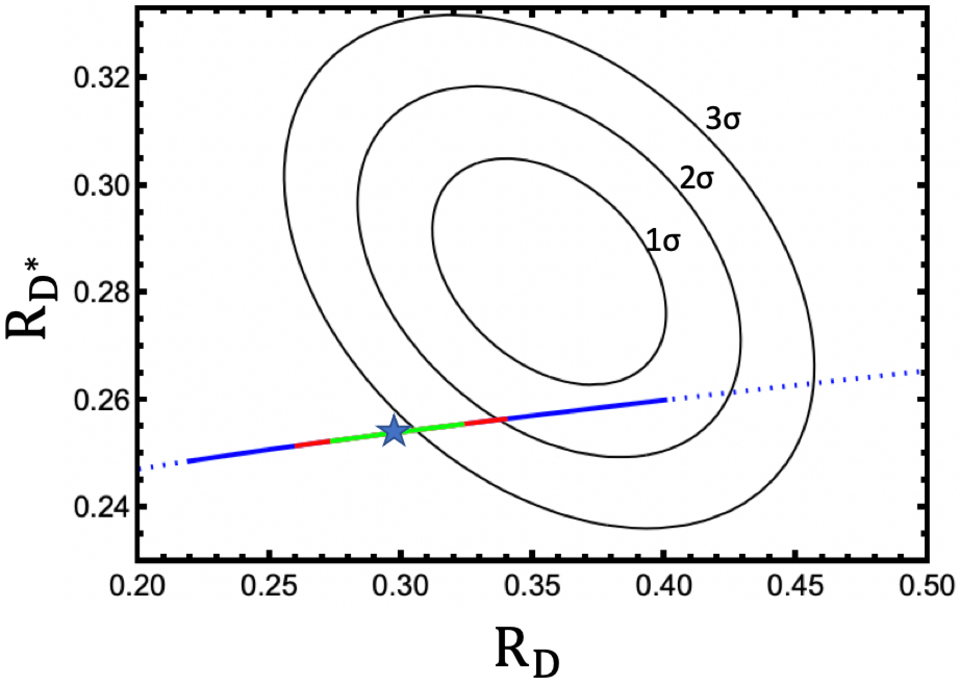
\includegraphics[width=0.5 \textwidth]{Figs/RD_V2.pdf}
\end{center}
 \caption{
Correlation between $R_{D^{(*)}}$ and BR($B_s\to \tau\ov \tau$) is shown.
Colored lines are prediction of $\rm{V}_2$ LQ model. 
The star mark corresponds to the SM prediction.
Blue dotted lines are excluded by the $B_s\to\tau\ov\tau$ measurement.
Blue solid lines (red solid lines) will be probed at Run\,3 (HL LHC). 
$1,\,2,\,3\sigma$ contours for $R_{D^{(*)}}$ are shown in black.
  \label{fig:RD_Bstautau}
 }
\end{figure}
%%%%%%%%%%%%%%%%%%%%%%%%%

It is noted that other LQ, $\text{S}_1$, $\text{R}_2$ and U(2) flavored $\text{U}_1$ do not contribute to a single scalar operator.
Given that $R_{D^{(*)}}$ anomaly is explained by $O_{S_R}$ in the $\rm{V}_2$ LQ scenario, the coupling product, $h_1^{33}\times h_2^{23}$, should be sizable. 
As shown in Eqs.\,(\ref{eq:ND_SL_ope2}) and (\ref{eq:Btotautau}), the sizable $h_1^{33}\times h_2^{23}$ enhances BR($B_s\to\tau\ov\tau$), so that it is a key prediction to test this model.
This correlation has not been pointed out in the previous works to our best knowledge.
In Fig.\,\ref{fig:RD_Bstautau}, we show the correlation between $R_{D^{(*)}}$ and BR($B_s\to\tau\ov\tau$).
The colored line is the model prediction.
Blue dashed region is excluded by the current $B_s\to\tau\ov\tau$ constraint.
Blue and red solid lines are expected to be probed at the Run\,3 and the HL LHC.
The green would not be uncovered.
We see that the Run\,3 and the HL LHC data will be the interesting probe of the 2\,$\sigma$ region.
For the SM prediction that is depicted by a star symbol, we adopt the latest HFLAV2023 average of $R_{D}=0.298$ and $R_{D^{*}}=0.254$.\footnote{It is noted if we rely on the Lattice predictions of $R_{D}=0.299$ and $R_{D^{*}}=0.265$ \cite{MILC:2015uhg,FermilabLattice:2021cdg,Fedele:2022iib}, where $R_{D^*}$ is shifted by 0.01, the model prediction goes through the 1\,$\sigma$ region. 
On the other hand, if we adopt $R_{D}=0.290$ and $R_{D^{*}}=0.248$ \cite{Iguro:2020cpg} where the form factor is also fitted also with full angular data from the Belle \cite{Belle:2017rcc,Belle:2018ezy}, the $\rm{V}_2$ prediction contour goes though the 2\,$\sigma$ region.}


The same semitauonic scalar operator which again corresponds to the category (iv) largely enhances $B_c\to\tau\ov\nu_\tau$ branching ratio.
Although $R_{D^*}$ is not largely deviated from the SM prediction, $R_{D^*}$ and BR$(B_c\to\tau\ov\nu_\tau)$ has a correlation:
\begin{align}
 \label{eq:Bc}
{\rm{BR}}(B_c\to \tau\overline\nu_\tau) ={\rm{BR}}(B_c\to \tau\overline\nu_\tau)_{\rm SM}\left| 1 + \frac{m_{B_c}^2}{m_b+m_c}C_{S_R}^{cb} \right|^2 ,    
\end{align}
where BR$(B_c\to \tau\overline\nu_\tau)_{\rm SM} \simeq 0.022$ \cite{Iguro:2022yzr}.
In the numerical evaluation, $m_b=4.18$\,GeV and $m_c(m_b)=0.92$\,GeV are used.
The upper bound of the coupling product from  BR$(B_s\to\tau\ov\tau)$ indirectly set that of ${\rm{BR}} (B_c\to\tau\ov\nu_\tau)$ as
\begin{align}
{\rm{BR}} (B_c\to\tau\ov\nu) \le 8\,\%.
\end{align}
This satisfies the current conservative limit, ${\rm{BR}} (B_c\to\tau\ov\nu_\tau) \lesssim 60\,\%$ \cite{Blanke:2018yud} while future lepton colliders can test the SM prediction at $\mathcal{O}(1)\,\%$ accuracy \cite{Zheng:2020ult,Amhis:2021cfy,Fedele:2023gyi}.


The coupling product also contributes to $B_s\to K \tau\ov\tau$ corresponding to the category (i).
The current limit announced by the BaBar collaboration is BR$(B_s\to K \tau\ov\tau)\le 2.25\times 10^{-3}$ \cite{BaBar:2016wgb} where the SM prediction is $\mathcal{O}(10^{-7})$ \cite{Capdevila:2017iqn}.
Unlike $B_s\to\tau\ov\tau$ and $B_c\to\tau\ov\nu_\tau$, the enhancement is not significant due to a lack of the chirality enhancement and hence we skip this channel.


%%%%%%%%%%%%%%%%%%%%%%%%%%%%%%%%%%%%%%%%%%%%%%%%%%%%%%%%%%%%
\subsection{LHC phenomenology at $\mathcal{O}(\epsilon^0)$ }
\label{sec:LHC}
%%%%%%%%%%%%%%%%%%%%%%%%%%%%%%%%%%%%%%%%%%%%%%%%%%%%%%%%%%%%
%%%%%%%%%%%%%%%%%%%%%%%%%
\begin{figure}[t]
\begin{center}
 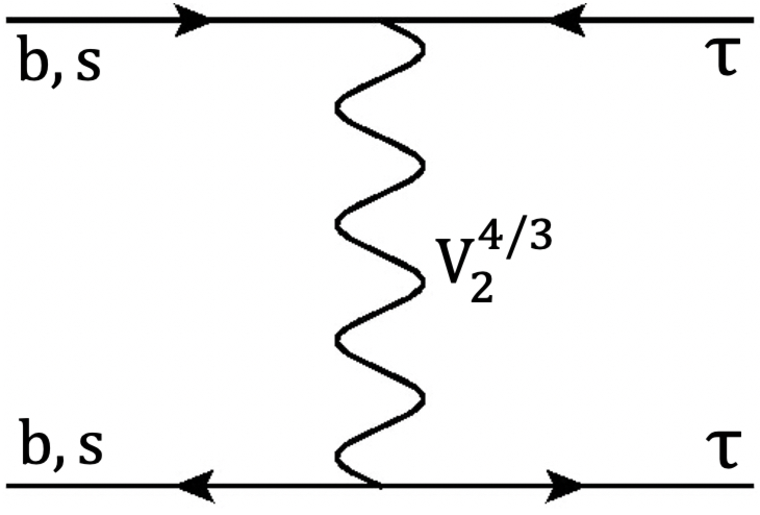
\includegraphics[width=0.3 \textwidth]{Figs/dia_LHC_4o3.pdf}~~~~~~~~~~
  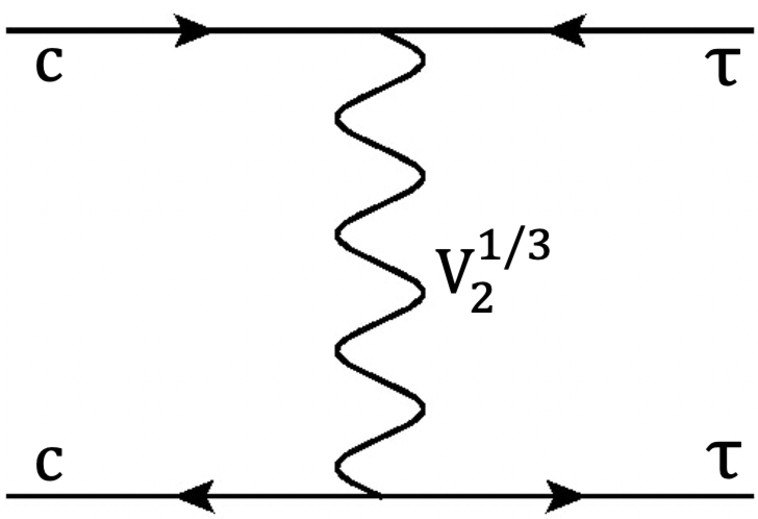
\includegraphics[width=0.3 \textwidth]{Figs/dia_LHC_1o3.pdf}
\end{center}
 \caption{
The contributing Feynman diagrams for $\tau\ov\tau$ final state at the LHC.
Both $\rm{V}^{4/3}_2$ (left) and $\rm{V}^{1/3}_2$ (right) contribute to the high-$p_T$ signature.
  \label{fig:diagrams}
 }
\end{figure}
%%%%%%%%%%%%%%%%%%%%%%%%%

Since the LQ has a TeV-scale mass, the direct search at the LHC is a powerful tool to probe the scenario. $\rm{V}_2$ is pair-produced by the strong interaction at the hadron collider. Depending on the subsequent decays, we can set the lower limit on the $\rm{V}_2$ mass.
The sizable $h_{1}^{33}$ and $h_{1}^{23}$ respectively lead the following decays:  $\rm{V}^{1/3}_2\to b\nu_\tau$, $\rm{V}^{4/3}_2\to b\tau$, $\rm{V}^{1/3}_2\to c\tau$ and $\rm{V}^{4/3}_2\to s\tau$.
The LQ mass has been directly constrained as $M_\text{LQ} \gtrsim 1.5\,\text{TeV}$ from the searches for the LQ pair-production~\cite{Sirunyan:2018vhk,Aaboud:2019bye,Aad:2021rrh,ATLAS:2021jyv}. 
Furthermore, it is known that the high-$p_T$ region is important to prove the new physics scenario that explains the $R_{D^{(*)}}$ anomaly \cite{Faroughy:2016osc,Iguro:2018fni,Mandal:2018kau,Greljo:2018tzh,Altmannshofer:2017poe,Iguro:2017ysu,Abdullah:2018ets,Marzocca:2020ueu,Iguro:2020keo,Endo:2021lhi}.
In our model, $\rm{V}^{4/3}_2$ also contributes to the di-$\tau$ final state, so that the searches for di-$\tau$ with high-$p_T$ \cite{CMS:2022goy,ATLAS:2020zms} provide the better probe than the $\tau\nu$ searches studied in Refs. \cite{CMS:2015hmx,Aaboud:2018vgh,Sirunyan:2018lbg,ATLAS:2021bjk}. 
See Fig.\,\ref{fig:diagrams} for the contributing Feynman diagrams.
We study the bounds from the  di-$\tau$ and mono-$\tau$ signatures at the LHC.
We constructed the $\chi^2$ function based on the high-$p_T$ bins of Refs.\,\cite{ATLAS:2020zms,ATLAS:2021bjk}
using HighPT \cite{Allwicher:2022mcg} as a function of couplings and draw the upper bounds on the LQ couplings where $m_{\rm{V}_2}=2\,$TeV is fixed.
It is found that the mediator mass dependence in di-$\tau$ final state is mild in terms of the four-fermi interactions.
We note that the study of the interplay between $R_{D^{(*)}}$ and collider physics in this model has not been done before.
%%%%%%%%%%%%%%%%%%%%%%%%%
\begin{figure}[t]
\begin{center}
 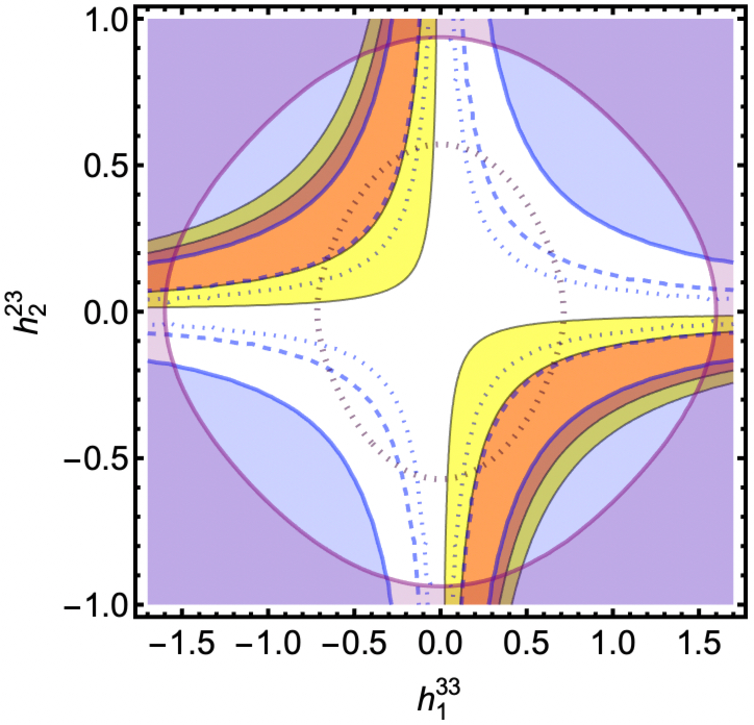
\includegraphics[width=0.45 \textwidth]{Figs/h133h223_min.pdf}
\end{center}
 \caption{
$R_{D^{(*)}}$ favored region, constraint from $B_s\to\tau\ov\tau$ and di-$\tau$ searches at the LHC are shown on $h_1^{33}$ vs. $h_2^{23}$.
We fixed the $\rm{V}_2$ LQ mass to 2\,TeV.
Orange and yellow regions correspond to $\chi^2\le6.18$ (orange) and $\chi^2\le11.83$ (yellow) for the $R_{D^{(*)}}$ data, respectively.
Blue shaded region is excluded by the current $B_s\to\tau\ov\tau$ and dashed and dotted contours denote the future prospect for the Run 3 and HL LHC.
Purple shaded region is also excluded by the high-$p_T$ di-$\tau$ searches at the LHC.
The future projection is shown in the dotted contour.
  \label{fig:h133_h223}
 }
\end{figure}
%%%%%%%%%%%%%%%%%%%%%%%%%

In Fig.\,\ref{fig:h133_h223} solid and dotted purple lines show the current bound and future prospect of the LHC experiment, respectively.
The shaded region is excluded.
We overlaid the current constraint and future sensitivity of the Run\,3 and the HL LHC from $B_s\to\tau\ov\tau$ with solid, dashed and dotted blue lines.
The regions favored by $R_{D^{(*)}}$ are shown in orange and yellow: $\chi^2\le6.18$ (orange) and $\chi^2\le11.83$ (yellow).
We see that the Run\,3 $B_s\to\tau\ov\tau$ will test the whole orange region and at the HL LHC, both high-$p_T$ and the B-factory probe the remaining interesting parameter region. 


We briefly summarize the difference in the prediction of the other LQ scenarios:
\begin{itemize}
\item {BR($B_s\to\tau\ov\tau$) is largely enhanced, while, for instance, it is not in the $\rm{S}_1$ LQ case.
Although $\rm{R}_2$ and U(2) flavored $\rm{U}_1$ LQ enhance BR($B_s\to\tau\ov\tau$), the former (latter) has $C_T$ ($C_{V_L}$) contribution in $R_{D^{(*)}}$ too. 
Therefore the degree of the enhancement in BR($B_s\to\tau\ov\tau$) is mild for the other LQs.
Since the coupling strength to explain the deviation is larger than the $\rm{U}_1$ LQ model, we can test this scenario with smaller amount of the data.} 
\item {Furthermore, as is shown in Ref.\,\cite{Iguro:2018vqb}, polarization observables in $\Bb\to D^{(*)} \tau\ov\nu_\tau$ are helpful to distinguish those scenarios.
Especially $\tau$ polarization will be a key observable.}
\item {The larger signal rate in di-$\tau$ is predicted at the LHC, compared to the $\rm{U}_1$ LQ.
This is because that the larger couplings are necessary to explain $R_{D^{(*)}}$, and both $\rm{V}^{4/3}_2$ and $\rm{V}^{1/3}_2$ contribute to the processes.
Therefore the LHC data in high-$p_T$ di-$\tau$ channel will be very important to probe the model.}
\end{itemize}


%%%%%%%%%%%%%%%%%%%%%%%%%%%%%%%%%%%%%%%%%%%%%
\subsection{Flavor phenomenology at $\mathcal{O}(\epsilon^0)$ and $\mathcal{O}(\lambda^1)$ }
\label{sec:next_to_minimal_flavor}
%%%%%%%%%%%%%%%%%%%%%%%%%%%%%%%%%%%%%%%%%%%%%
%%%%%%%%%%%%%%%%%%%%%%%%%
\begin{figure}[t]
\begin{center}
 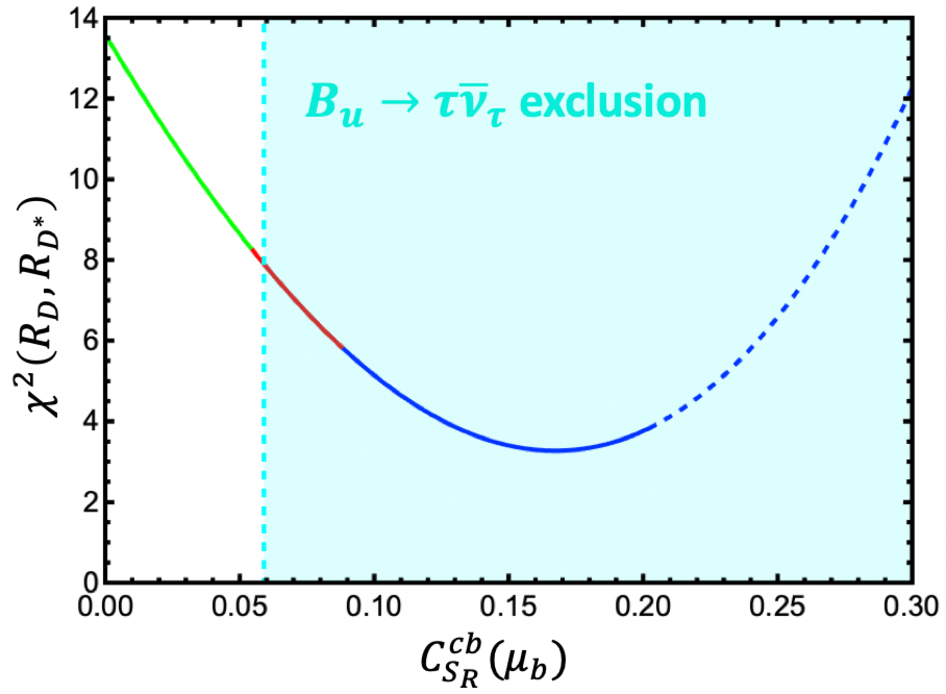
\includegraphics[width=0.5 \textwidth]{Figs/RDvsBtaunu.pdf}
\end{center}
 \caption{
$\chi^2(R_D,\,R_{D^{*}})$ and $R_{B_u}$ as a function of $C_{S_R}^{cb}(\mu_b)$.
$C_{S_R}^{cb}=(0.88+2.45i)C_{S_R}^{ub}$ is fixed for $R_{B_u}$. The meaning of the color is the same as in Fig.\,\ref{fig:RD_Bstautau}.
The blue dashed line is excluded by the current bound from $B_s\to\tau\ov\tau$.
The shaded cyan region is excluded by the current $B_u\to\tau\ov \nu_\tau$.
\label{fig:RD_Btaunu}
}
\end{figure}
%%%%%%%%%%%%%%%%%%%%%%%%%

The leptonic $B$ meson decay, $B_u\to \tau\ov\nu_\tau$, also constrain our model.\footnote{ This constraint has not been pointed out in the previous work \cite{Cheung:2022zsb}.}
This decay is enhanced by the scalar operator, although it is suppressed by an off-diagonal CKM element.
Similar to the $B_c$ decay, we can derive the numerical formula as 
\begin{align}
 \label{eq:Bu}
{\rm{BR}}(B_u\to \tau\overline\nu_\tau) ={\rm{BR}}(B_u\to \tau\overline\nu_\tau)_{\rm SM}\left| 1 + 3.75 C^{ub}_{S_R} \right|^2.
\end{align}
The SM prediction is estimated as BR$(B_u\to \tau\ov\nu_\tau)_{\rm SM}\simeq 0.95 \times 10^{-4}$ with $|V_{ub}|=0.409\times 10^{-2}$.\footnote{This is the average of inclusive and exclusive $V_{ub}$.}
$C_{S_R}^{ub}$ at the LQ scale is estimated as
\begin{align}
    C_{S_R}^{ub}(\mu_{\rm{LQ}})\simeq(0.15+0.44i)\left(\frac{2\,{\rm{TeV}}}{m_{\rm{V}_2}}\right)^2\left(\frac{h_1^{33}h_2^{23*}}{-0.5}\right).
    \label{eq:eq:CSRub}
\end{align}
It is noted that the coefficient in Eq.\,(\ref{eq:eq:CSRub}) is bigger than that of Eq.\,(\ref{eq:eq:CSRcb}) because of the factor of $(V_{cb} V_{us})/V_{ub}=0.84+2.46i$.

The current experimental world average is BR$(B_u\to \tau\overline\nu_\tau)=(1.09\pm0.24)\times 10^{-4}$ \cite{PDG2022}.
There is a notorious discrepancy between the inclusive and the exclusive determinations:
$|V_{ub}|_{\rm{inc}}=4.25\,(1\pm0.07)\times 10^{-3}$ and  $|V_{ub}|_{\rm{exc}}=3.70\,(1\pm0.04)\times 10^{-3}$. 
Therefore, we assign $14\,\%$ uncertainty to the SM amplitude.
On the other hand, the experimental result has $22\%$ uncertainty.
Combining those uncertainties at $2\sigma$, we allow $70\%$ uncertainty and set the following criteria:
\begin{align}
R_{B_u}=\frac{{\rm{BR}}(B_u\to \tau\ov\nu_\tau)}{{\rm{BR}}(B_u\to \tau\ov\nu_\tau)_{\rm{SM}}}\le1.7.
\label{eq:Butaunu_current}
\end{align}
It is noted that the following observables, 
\begin{align}
    R_{pl}=\frac{{\rm{BR}}(B_u\to\tau\ov\nu_\tau)}{{\rm{BR}}(B_u\to\mu\ov\nu_\mu)},~~~R_{ps}=\frac{\Gamma(B_u\to\tau\ov\nu_\tau)}{\Gamma(B_d\to\pi^+l\ov\nu_l)}
\end{align}
are free from $V_{ub}$ and useful to test the NP \cite{Tanaka:2016ijq}. The corresponding SM predictions are $R_{pl}^{\rm{SM}}=222$ and $R_{ps}^{\rm{SM}}=0.54\pm0.04$.\footnote{The large part of the uncertainty comes from $B\to \pi$ transition form factor \cite{Tanaka:2016ijq}.}
The current experimental constraint is given as $R_{ps}^{\rm{exp}}=0.73\pm0.14$ while $R_{ps}$ is not measured due to the large uncertainty in BR$(B_u\to\mu\ov\nu_\mu)$ \cite{Kou:2018nap}.
At $2\,\sigma$ level, this leads to $R_{B_u}\lesssim 2$, that is weaker than the constraint in Eq.\,(\ref{eq:Butaunu_current}).

The Belle II with 50\,ab$^{-1}$ of the data will measure  $R_{pl}$ and $R_{ps}$ at $12\,\%$ and $7\,\%$ at $1\,\sigma$.
Even if we adopt the current theoretical uncertainty for $R_{ps}$ to be conservative, we obtain the similar uncertainty.
It is noted that in our model, the modification of the denominator mode is negligible and hence the uncertainty of the ratio corresponds to the sensitivity to BR$(B_u\to\tau\ov\nu_\tau)$. 

In Fig.\,\ref{fig:RD_Btaunu} we show $\chi^2$ for $R_{D}$ and $R_{D^*}$.
The meaning of color and style of lines are the same as in Fig.\,\ref{fig:RD_Bstautau}.
The current conservative exclusion of Eq.\,(\ref{eq:Butaunu_current}) is shown in cyan region.
It is seen that $B_u\to\tau\ov\nu_\tau$ is more sensitive to $h_1^{33}\times h_2^{23*}$ than $B_s\to\tau\ov\tau$. 
This figure clearly shows that the interesting parameter space is already excluded by the current result of $R_{B_u}$. 
This bound, however, can be relaxed by sizable other LQ couplings, as discussed in Sec.\,\ref{sec:Oepsilon}. 


%%%%%%%%%%%%%%%%%%%%%%%%%%%%%%%%%%%%%%%%%%%%%%%%%%%%%%%%
\subsection{$\mathcal{O} (\epsilon)$ phenomenology}
\label{sec:Oepsilon}
%%%%%%%%%%%%%%%%%%%%%%%%%%%%%
%%%%%%%%%%%%%%%%%%%%%%%%%
\begin{figure}[t]
\begin{center}
 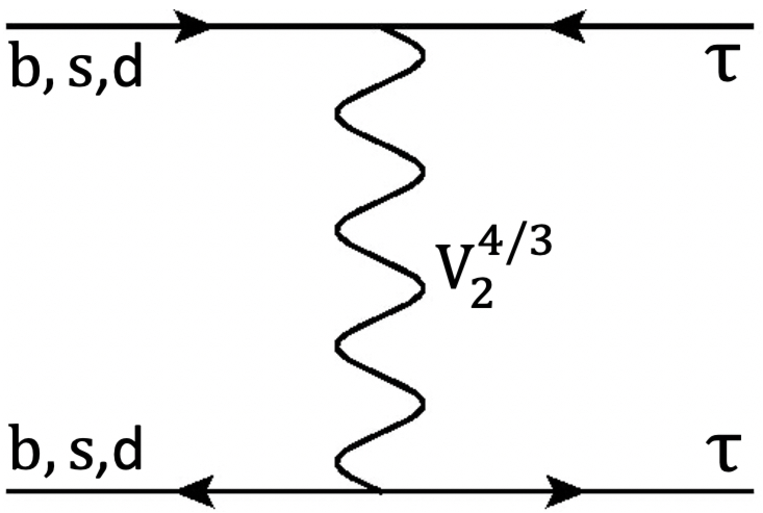
\includegraphics[width=0.3 \textwidth]{Figs/dia_LHC_4o3_v2.pdf}~~~~~~~~~~
  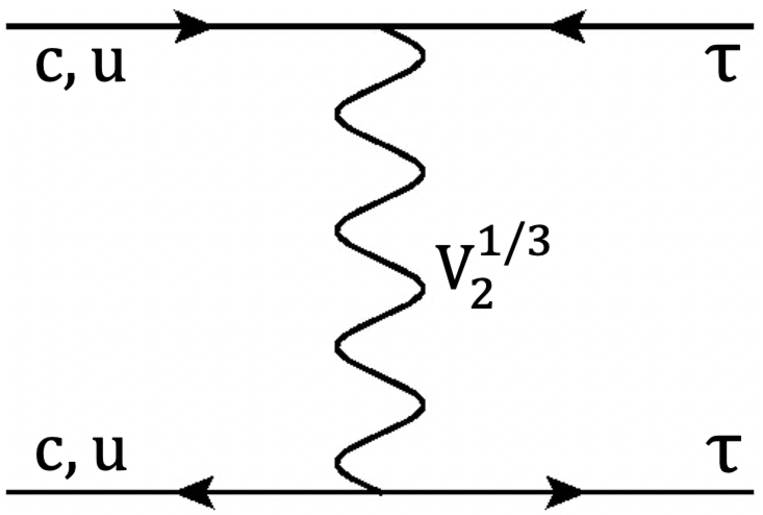
\includegraphics[width=0.3 \textwidth]{Figs/dia_LHC_1o3_v2.pdf}
\end{center}
 \caption{
  \label{fig:diagrams2}
  The contributing Feynman diagrams for $\tau\ov\tau$ final state at the LHC in the presence of non-vanishing $h_2^{13}$, $h_2^{23}$, $h_1^{33}$.
  In addition the one in Fig.\,\ref{fig:diagrams}, $h_2^{13}$ induces $d \ov d\to \tau \ov\tau$ and $u\ov u\to \tau\ov\tau$ processes mediated by $\rm{V}^{4/3}_2$ and $\rm{V}^{1/3}_2$.
 }
\end{figure}
%%%%%%%%%%%%%%%%%%%%%%%%%
In this section, we investigate $\mathcal{O} (\epsilon)$ contributions and derive the upper limit on the coupling products.
As is summarized in Tab.\,\ref{Tab:ModelNRC}, there are several processes to be discussed.
%%%%%%%%%%%%%%%%%%%%%%%%%%%%%%%%%%%%%%%%%%%%%%%%%%%%%%

First, we consider $h_2^{13}$ contribution. If $h_2^{13}$ is sizable, the coupling contributes to $B_u\to\tau\ov\nu_\tau$.  
The contribution to $C_{S_R}^{ub}$ is expressed as 
\begin{align}
C_{S_R}^{ub}(\mu_{\rm{LQ}})= -\frac{1}{\sqrt{2}G_F V_Q^{cb}}\frac{h_1^{33}\left(V_Q^{11}h_2^{13*}+V_Q^{12}h_2^{23*}\right)}{m_{\rm{V}_2}^2}.
\end{align}
If $h_2^{13*}=-V_Q^{12}/V_Q^{11}h_2^{23*}\simeq -0.23h_2^{23*}$ is satisfied, $C_{S_R}^{ub}$ can be enough small to evade the bound from $R_{B_u}$ mentioned above and rescue the solution.

The tree-level exchange of the LQ induces $B_d\to \tau \ov\tau$, and the amplitude is proportional to $h_1^{33} \times h_2^{13*}$.
The $B_d\to \tau\ov\tau$ contribution has a chirality enhancement, so that it gives a strong bound.
The current experimental upper limit is BR($B_d\to\tau\ov\tau)\le 2.1 \times 10^{-3}$ at 95\,$\%$ CL. \cite{PDG2022} and the Belle II experiment is expected to probe BR($B_d\to\tau\ov\tau)\simeq 9.6 \times 10^{-5}$ \cite{Kou:2018nap}.
We note that $B\to\pi\tau\ov\nu_\tau$ is also induced by the same operator but the bound is weak. 
In addition, $c\ov u\tau\ov \tau$ and $s\ov d\tau\ov\tau$ four-fermi interactions are lead by the tree-level LQ exchange 
and the coefficients are proportional to $h_2^{13} \times h_2^{23*}$.
The couplings, however, do not predict rare meson decays since $\tau$ mass does not allow decay processes such as $D\to\tau\ov\tau$ nor $D\to \pi \tau\ov\tau$.\footnote{The one-loop contribution contributes to $K-\ov{K}$ mixing, but the abound is not so tight since there is no chirality enhancement as long as $h_1^{13}\times h_1^{23*}$ is small.
Furthermore for the correct loop calculation, we need the UV model and hence we limit ourselves to focus on the tree level phenomenology in this paper. 
We will come back to this point in Sec.\,\ref{sec:Summary}.}


Our numerical analysis shows that the $R_{D^{(*)}}$ anomaly can be explained within 2$\,\sigma$, if $h_1^{33}\times h_2^{23*}$ is fixed within $[-0.29,\,-0.12]$ when $m_{\rm{V}_2}=2\,$TeV.
Let us define the ratio of $h_2^{13}$ to $h_2^{23}$ as $h_2^{13}=-\lambda^{uc} h_2^{23}$.
This ratio is limited by $B_u\to\tau\ov\nu_\tau$.
When $h_1^{33}\times h_2^{23*}$ is around $-0.29$ ($-0.12$),
$\lambda^{uc}$ should satisfy $0.07\lesssim\lambda^{uc}\lesssim 0.57$ ($0.16\lesssim\lambda^{uc}\lesssim 0.37$) to evade the $B_u\to\tau\ov\nu_\tau$ bound.
In the future, the Belle II experiment could improve the bound and this range could be reduced to be $0.20\lesssim\lambda^{uc}\lesssim 0.34$ ($0.16\lesssim\lambda^{uc}\lesssim 0.48$) if the experimental central value does not change \cite{Kou:2018nap}.

%%%%%%%%%%%%%%%%%%%%%%%%%
\begin{figure}[t]
\begin{center}
 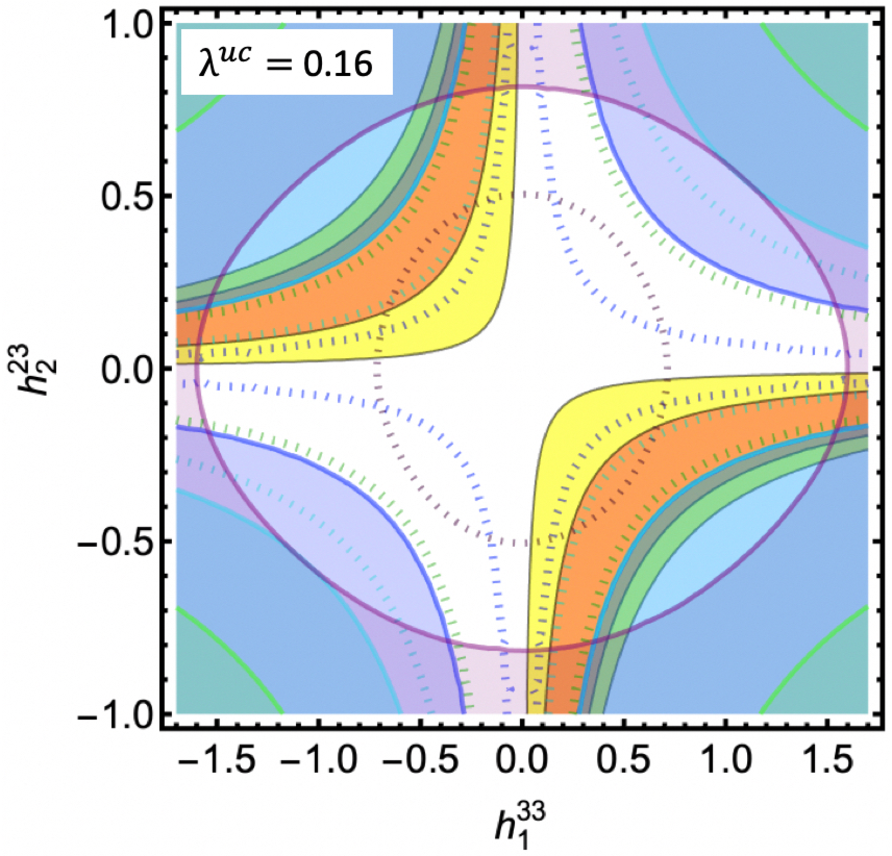
\includegraphics[width=0.32 \textwidth]{Figs/h133h223_m016.pdf}~~
 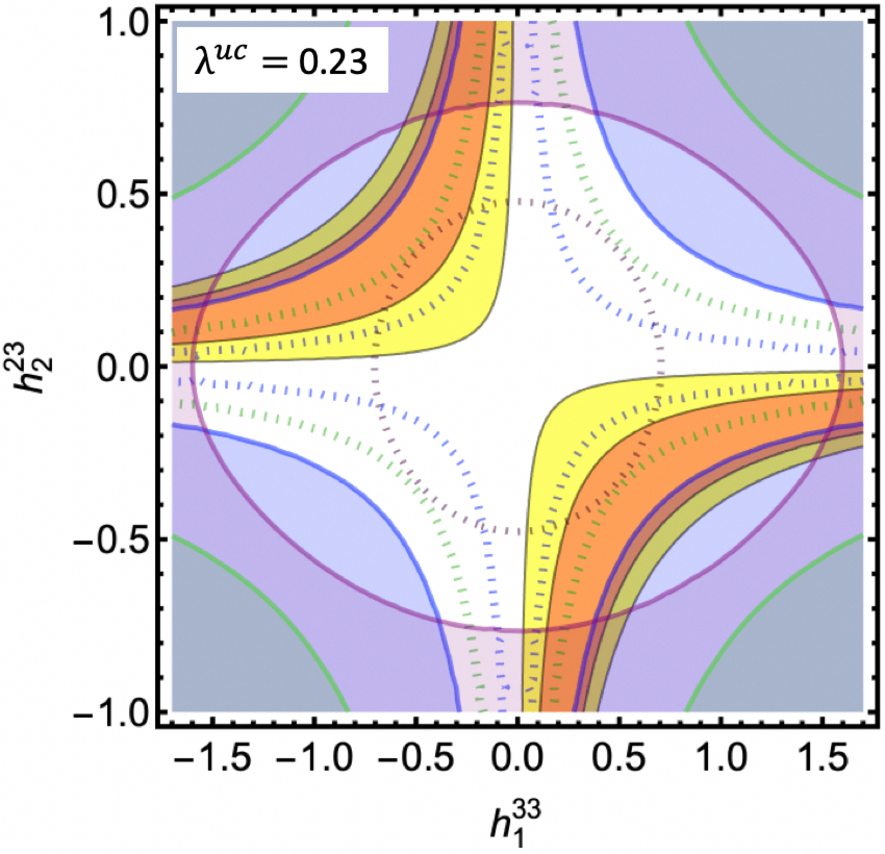
\includegraphics[width=0.32 \textwidth]{Figs/h133h223_m023.pdf}~~
 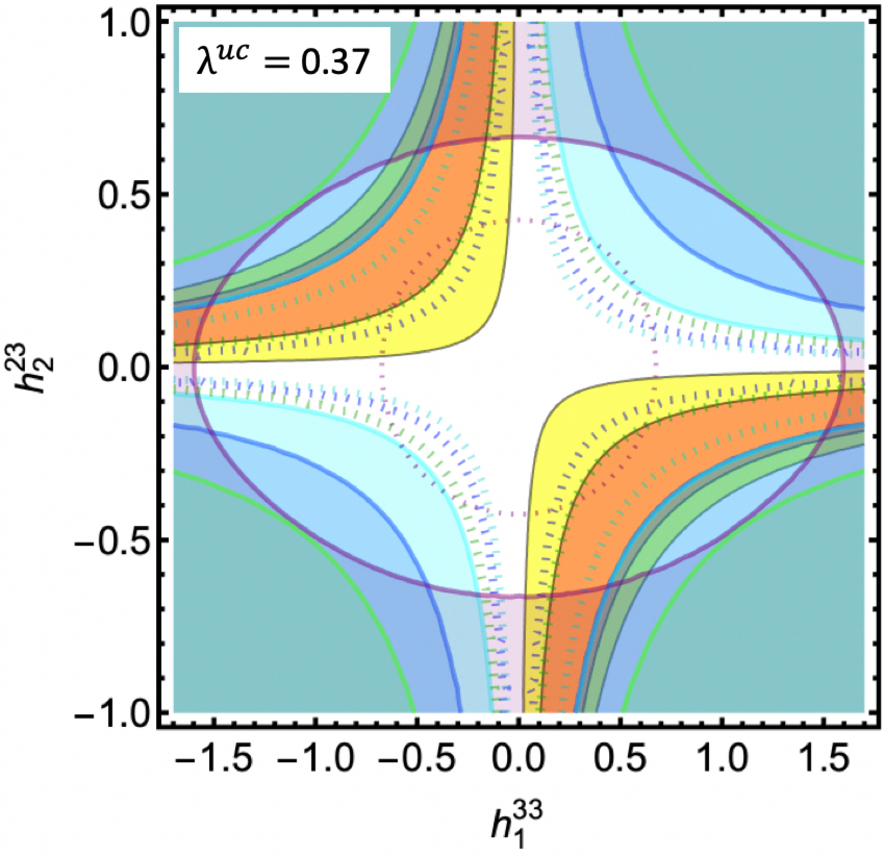
\includegraphics[width=0.32 \textwidth]{Figs/h133h223_m037.pdf}
\end{center}
 \caption{
  \label{fig:h133h223h213}
  The color code is the same as in Fig.\,\ref{fig:h133_h223}.
  Additionally, cyan and light green regions show the exclusion from $B_u\to\tau\ov\nu_\tau$ and $B_d\to\tau\ov\tau$.
  Their future prospects are also shown in dotted lines.
  }
\end{figure}
%%%%%%%%%%%%%%%%%%%%%%%%%
$h_2^{13*}$ also contributes to $C_{S_R}^{cb}$ as
\begin{align}
C_{S_R}^{cb}(\mu_{\rm{LQ}})= -\frac{1}{\sqrt{2}G_F V_Q^{ub}}\frac{h_1^{33}\left(V_Q^{22}h_2^{23*}+V_Q^{21}h_2^{13*}\right)}{m_{\rm{V}_2}^2},
\end{align}
although it is suppressed by $V_Q^{21}$.
Besides, $h_2^{13}$ also contributes to $d\ov d\to \tau\ov\tau$ and $u\ov u\to \tau\ov\tau$ processes at the LHC as shown in Fig.\,\ref{fig:diagrams2}.

In Fig.\,\ref{fig:h133h223h213}, $\lambda^{uc}$ is fixed at $\lambda^{uc}=0.16,\,0.23,\,0.37$ on the left, middle and right panels, respectively.
To see the prediction to motivate future experiments, the correlation among $\chi^2(R_D, R_{D^*})$, $R_{B_u}$, BR$(B_s\to\tau\ov\tau)\times 10^3$ and BR$(B_d\to\tau\ov\tau)\times 10^4$ is shown in Fig.\,\ref{fig:Obs_correlation}.
We see that in addition to $B_s\to\tau\ov\tau$, $B_d\to\tau\ov\tau$ plays an important role in the probe when $\lambda^{uc}=0.23$ and 0.37.
When $\lambda^{uc}=0.16$ and 0.37, the future $R_{B_u}$ measurement can probe the best fit point of the model.
On the other hand, $R_{B_u}$ is suppressed when $\lambda^{uc}=0.23$, because of the cancellation mentioned above.
%%%%%%%%%%%%%%%%%%%%%%%%%
\begin{figure}[t]
\begin{center}
 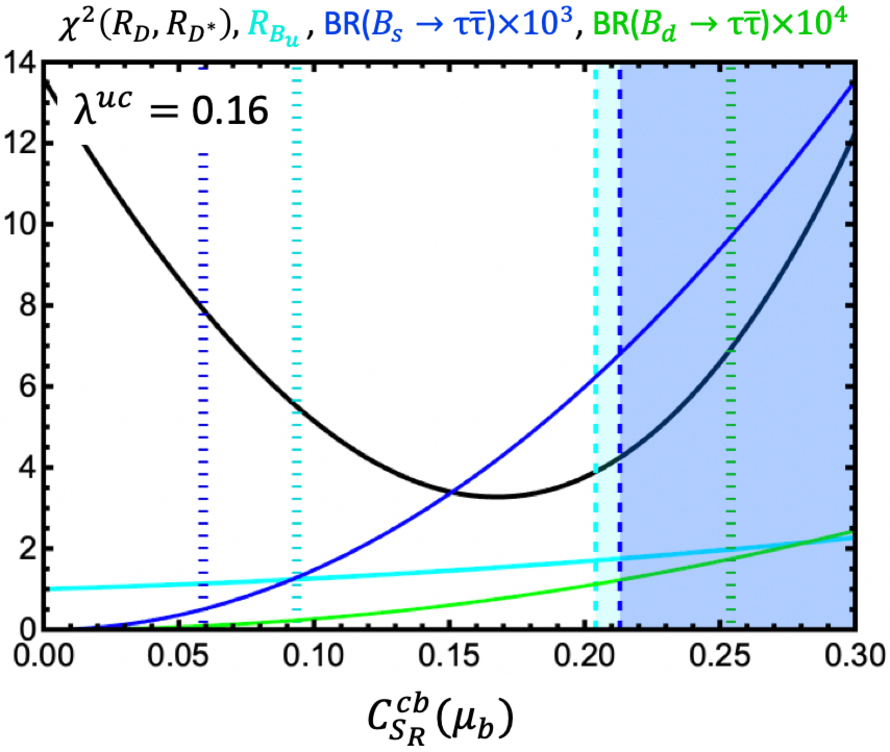
\includegraphics[width=0.32 \textwidth]{Figs/Obs016.pdf}~~
 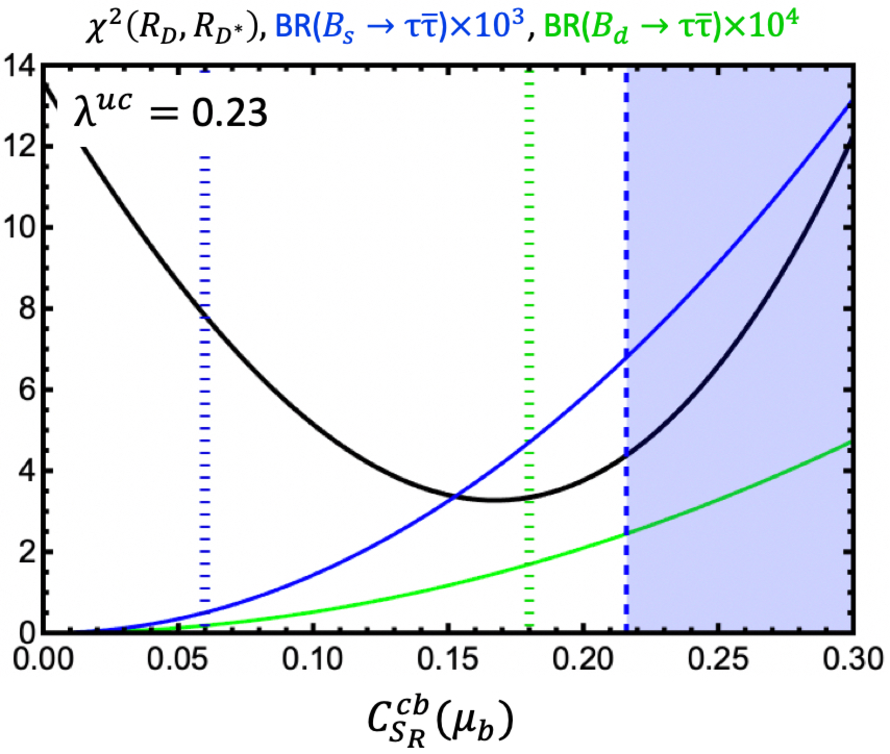
\includegraphics[width=0.32 \textwidth]{Figs/Obs023.pdf}~~
 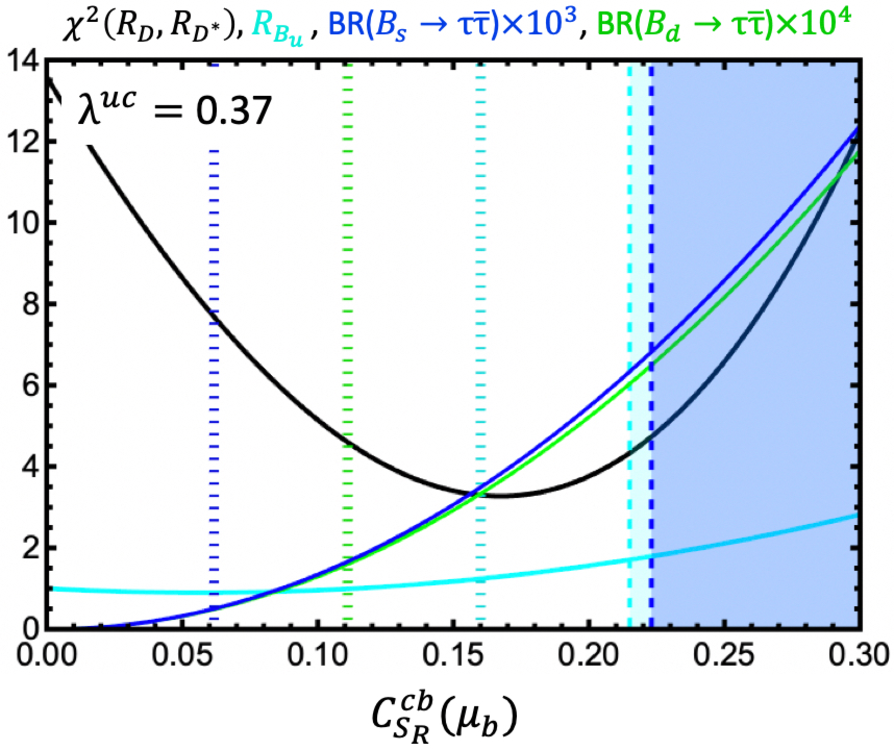
\includegraphics[width=0.32 \textwidth]{Figs/Obs037.pdf}
\end{center}
 \caption{
  \label{fig:Obs_correlation}
  The correlation of prediction is shown as a function of $C_{S_R}^{cb}(\mu_b)$ fixing $\lambda^{uc}=0.16$ (left), 0.23 (middle) and 0.37 (right).
  $\chi^2(R_D,\,R_{D^*})$, $R_{B_u}$ is shown in black and cyan.
  BR$(B_s\to\tau\ov\tau)\times 10^3$ and BR$(B_d\to\tau\ov\tau)\times 10^4$ are shown in blue and light green lines.
  The current exclusion is shown in each color.
  The future prospect is shown in dotted line.
  }
\end{figure}
%%%%%%%%%%%%%%%%%%%%%%%%%
We note that that real $h_1^{33}\times h_2^{23*}$ is favored by the current $R_{D^{(*)}}$ measurement.
If $h_1^{33}\times h_2^{13*}$ is also real, we obtain the prediction for $R_{B_u}$ as $0.89\lesssim R_{B_u}$, due to the relative phase between the SM amplitude and $\rm{V}_2$ amplitude.
We note that the collider reach is also mildly extended with the inclusion of non-vanishing $h_2^{13}$.

We investigate the phenomenological impact of other couplings.
As shown in Tab.\,\ref{Tab:ModelNRC}, sizable $h_1^{13}$ and $h_2^{23*}$ couplings
predict the contributions to the leptonic $D$ meson decays: $D_{d,s}\to\tau\ov\nu_\tau$, corresponding to the category (iv).
To study the bounds numerically, we define
\begin{align}
R_{D_d}=\frac{{\rm{BR}}(D_d\to \tau\ov\nu_\tau)}{{\rm{BR}}(D_d\to \tau\ov\nu_\tau)_{\rm SM}} =\left| 1 + 1.47 C^{cd}_{S_R} \right|^2 ,
\label{eq:D}
\end{align}
and
\begin{align}
 \label{eq:Ds}
R_{D_s}=\frac{{\rm{BR}}(D_s\to \tau\ov\nu_\tau)} {{\rm{BR}}(D_s\to \tau\ov\nu_\tau)_{\rm SM}}=\left| 1 + 1.72  C_{S_R}^{cs} \right|^2,
\end{align}
where BR$(D_d\to \tau\ov\nu_\tau)_{\rm SM}\simeq1.06 \times 10^{-3}$ and BR$(D_s\to \tau\ov\nu_\tau)_{\rm SM} \simeq 5.2 \times 10^{-2}$. The numerical estimations are obtained using $|V_{cd}|=0.221\pm0.004$, $|V_{cs}|=0.975\pm0.006$ \cite{PDG2022}, $f_{D}=0.2120\pm0.007$\,GeV and  $f_{D_s}=0.2499\pm0.005$\,GeV \cite{HFLAV:2022pwe}.
Compared to $B_u$ and $B_c$ decays, those enhancement factors are small where $m_c(m_c)=1.27$\,GeV is used. $C_{S_R}^{cs}$ is given by Eq. (\ref{eq:CSR_general}),
and proportional to $h_1^{13}\times h_2^{23*}$.

There are experimental results of those decays: BR$(D_d\to \tau\ov\nu_\tau)_{\rm exp}=(1.20\pm0.27)\times 10^{-3}$ and  BR$(D_s\to \tau\ov\nu_\tau)_{\rm exp}=5.32\pm0.11\,\%$ \cite{PDG2022}.
Furthermore, the BES III experiment reports the recent result \cite{BESIII:2019vhn}: BR$(D_d\to\tau\ov\nu_\tau)$/BR$(D_d\to\mu\ov\nu_\mu)=3.21(1\pm0.24)$ where the SM prediction is 2.67. 
When we require $C_{S_R}^{cs}$ to satisfy $0.5\le {\rm{BR}}(D_d\to \tau\ov\nu_\tau)/{\rm{BR}}(D_d\to \tau\nu_\tau)_{\rm{SM}}\le1.5$ and $0.95\le{\rm{BR}}(D_s\to \tau\ov\nu_\tau)/{\rm{BR}}(D_s\to \tau\nu_\tau)_{\rm{SM}}\le1.05$, we obtain 
\begin{align}
   -1.3 \lesssim h_1^{13}\times h_2^{23*}\lesssim 1.1,~~~ 
   -0.46 \lesssim h_1^{23}\times h_2^{23*}\lesssim 0.48.
\end{align}


Sizable $h_1^{13}$ and $h_1^{23}$ enhances or suppresses $B\to K^{(*)} \nu_\tau\ov\nu_\tau$ and $B\to \pi \nu_\tau\ov\nu_\tau$ corresponding to the category 
(ii).
The contributions of the LQ exchange are proportional to $h_1^{33}\times h_1^{23*}$ and $h_1^{33}\times h_1^{13*}$, respectively.\footnote{We find that $B\to K^{(*)} \tau\ov\tau$ and $B\to \pi \tau\ov\tau$ are less constraining compared to $B_s\to\tau\tau$ \cite{Capdevila:2017iqn}. In fact, the bound on $B\to \pi \tau\ov\tau$ is not available in PDG \cite{PDG2022}.
}
The LQ contributions correspond to the vector operators.
It is conventional to define the ratio as $\mathcal{R}_{M_1}^{\nu} = {\rm{BR}}(B\to M_1\nu\ov\nu )/{\rm{BR}}(B\to M_1 \nu\ov\nu )_{\rm{SM}}$.
The Belle collaboration has provided an upper bound as 
 $\mathcal{R}_{K^*}^{\nu} \le 2.7$ and $\mathcal{R}_{K}^{\nu } \le 3.9$ at the $90\%$ CL.~\cite{Belle:2017oht}.
The Belle II could measure the SM prediction with $10\,\%$ accuracy \cite{Kou:2018nap}.
Following Ref.\,\cite{Buras:2014fpa}, those ratios are expressed as 
\begin{align}
\mathcal{R}_{K^*}^{\nu} =(1-2\eta_{\nu})\epsilon_{\nu}^2,~~
\mathcal{R}_{K}^{\nu} =(1+\kappa_{\nu}\eta_{\nu\nu})\epsilon_{\nu}^2,
\end{align}
where
\begin{align}
\epsilon_{\nu}=\frac{\sqrt{|C_L^{\rm SM}|^2+|C_{R}^{bs}|^2}}{|C_L^{\rm SM}|},~~
\eta_{\nu}=\frac{-\rm{Re}\left( C_L^{\rm SM}C_{R}^{bs*} \right)}{|C_L^{\rm SM}|^2+|C_{R}^{bs}|^2},
\end{align}
and $\kappa_{\nu}= 1.34 \pm 0.04$ with $C_L^{\rm SM}\simeq-6.35\,$.
Similarly the current upper limit on $B\to \pi\nu\ov \nu$ is approximately given as 
\begin{align}
\mathcal{R}_{\pi}^{\nu}\lesssim 6000,
\end{align}
using the SM prediction of ${\rm{BR}}(B^0\to\pi^0 \nu\ov \nu)_{{\rm{SM}}}=(5.4\pm0.6)\times 10^{-8}$ \cite{Bause:2022rrs} and the current experimental constraint, ${\rm{BR}}(B^0\to\pi^0 \nu\ov \nu)\le0.9\times 10^{-5}$ at $90\,\%$ C.L. \cite{PDG2022}.
Those upper bounds lead to 
\begin{align}
   -0.27 \lesssim h_1^{33}\times h_1^{23*}\lesssim 0.21,~~
   -3.7 \lesssim h_1^{33}\times h_1^{13*}\lesssim 3.7.
\end{align}
We find that the constraints from $B_d\to\tau\ov\tau$ and $B_s\to\tau\ov\tau$ lead to $-1.8 \lesssim h_1^{33}\times h_1^{13*} \lesssim 1.8$ and $-2.65 \lesssim h_2^{33}\times h_2^{23*} \lesssim 2.65$.


The bounds on the coupling products are summarized 
in Tab.\,\ref{Tab:ModelNRC_summary}.
We see that there are several combinations that are allowed to be $\mathcal{O}(1)$.
Especially, it is not easy to constrain $h_1^{33}\times h_1^{13*}$, $h_2^{13}\times h_2^{23*}$ and $h_2^{33}\times h_2^{23*}$ using tree level processes.
In other words $h_{2}^{33}$ and $h_1^{13}$ can be of order 1 while $h_2^{13}$ and $h_1^{23}$ should be somewhat smaller.
We may obtain strong bounds considering one-loop contributions.
Such a higher-order contribution usually involves extra fields in the loop, so 
a concrete setup needs to be taken into account.

Finally, we discuss the bound from the collider experiments.
When $h_1^{13}$ and $h_2^{13}$, that correspond to the couplings involving light quarks, are sizable, our model 
can be constrained by the collider searches further.
We study the bounds from the di-$\tau$ and mono-$\tau$ signatures at the LHC by repeating the procedure explained in Sec.\,\ref{sec:LHC}.
As shown in Figs.\,\ref{fig:diagrams2}, the t-channel diagrams given by the exchange of the LQ induce di-$\tau$ signatures.
Analogously we have t-channel diagrams contributing to mono-$\tau$ signature.
Based on Run\,2 full data  we derive the upper limit on the coupling at $2\sigma$ as follows :
\begin{eqnarray}
|h_1^{13}|\le0.55,&& |h_2^{13}|\le0.51,~ |h_1^{23}|\le1.01,~ |h_2^{23}|\le0.93, \nonumber \\ |h_1^{33}|\le1.60,&& |h_2^{33}|\le1.66.
\end{eqnarray}
In this analysis, we turn on the only one coupling assuming that the other couplings are vanishing.
We see that $h_{1,2}^{13}$ coupling can be at most 0.5.
Also we can set the upper limit on the least constrained $h_2^{33}$ with LHC data.
This collider constraint is complementary to the flavor constraint.
We introduce a Yukawa texture, that respects the $\tau$ number, as an illustration:\footnote{We note that $h^{33}_{2}$ could be sizable as shown in Table \ref{Tab:ModelNRC_summary}.}
\begin{eqnarray}
  h_1^{ij} \simeq\left(
  \begin{array}{ccc}
   ~0~&~0~&~\mathcal{O}(10^{-3})\\
   ~0~&~0~&~\mathcal{O}(10^{-2})\\
   ~0~&~0~&~\mathcal{O}(1)\\
  \end{array}
  \right),~~~h_2^{ij} \simeq\left(
  \begin{array}{ccc}
   ~0~&~0~&~-0.23 h_2^{23}\\
   ~0~&~0~&~\mathcal{O}(1)\\
   ~0~&~0~&~\mathcal{O}(0.1) \\
  \end{array}
  \right).
\label{eq:coupling_structure_2023}
\end{eqnarray}
%%%%%%%%%%%%%%%%%%%%%%%%%%%%%%%%%%%%%%%%%%%%%%%%%%%%%%%%%%%%%%%
\begin{table}[t]
\begin{center}
\scalebox{0.95}{
  \begin{tabular}{c|c} \hline
   Coupling product & bound \\ \hline \hline 
 $h_1^{33}\times h_2^{23*}$ &   [$-0.28,~-0.12$]\\ \hline\hline
  $h_1^{33}\times h_2^{13*}$ &  [$-0.02,~0.04$] \\  \hline
  $h_1^{33}\times h_2^{33*}$ &  --- \\ \hline
  $h_1^{33}\times h_1^{13*}$ &  [$-1.8,~1.8$] \\ \hline
  $h_1^{33}\times h_1^{23*}$ &  [$-0.27,~0.21$] \\ \hline
  $h_1^{13}\times h_2^{23*}$ & [$-1.3,~1.1$] \\ \hline
  $h_1^{23}\times h_2^{23*}$ &  [$-0.46,~0.48$] \\ \hline
  $h_2^{13}\times h_2^{23*}$ &  --- \\ \hline
  $h_2^{33}\times h_2^{23*}$ &  [$-2.65,~2.65$] \\ \hline
   \end{tabular}
  }
  \caption{Summary table for the non-LHC bound on the coupling product assuming $m_{\rm{V}_2}=2\,$TeV.
}
  \label{Tab:ModelNRC_summary}
\end{center}   
\vspace{-.45cm}
\end{table}
%%%%%%%%%%%%%%%%%%%%%%%%%%%%%%%%%%%%%%%%%%%%%%%


%%%%%%%%%%%%%%%%%%%%%%%%%%%%%%%%%%%%%%%%%%%%%%%%%%%%%%%%
\section{Summary and discussion}
\label{sec:Summary}
%%%%%%%%%%%%%%%%%%%%%%%%%%%%%
In this paper we studied phenomenology of the model with isodoublet vector LQ, $\rm{V}_2$.
In light of the recent result of $R_{D^{(*)}}$, the LQ becomes very interesting.
$\chi^2(R_D,\,R_{D^*})$ can be as small as 3.7 in this model and the minimal coupling scenario predicts that $B_s\to\tau\ov\tau$ is within the reach of the Run\,3 LHCb measurement. 
In the minimal setup, $B_u\to\tau\ov\nu_\tau$ is deviated from the SM prediction, so that the setup is excluded.
This bound can be evaded by introducing another flavor violating coupling to the large contribution to $B_u\to\tau\ov\nu_\tau$.
We conclude that there are setups that are consistent with the experimental results related to the flavor physics as well as the high-$p_T$ signals.


We only discussed the tree-level contributions induced by the $\rm{V}_2$ exchange.
The LQ mass is not large, so it may be necessary to take into account the one-loop corrections involving $\rm{V}_2$. The study, however, would requires a complete model since the loop diagrams involve extra fields e.g. extra fermions and scalars in general and the contributions would not be negligible \cite{Iguro:2022ozl}. 
It would be challenging to construct a complete model with $\rm{V}_2$, since the constraint from the lifetime of proton is very strong and a specific parameter setup is required to explain the $R_{D^{(*)}}$ anomaly.
The quantum number of $\rm{V}_2$ is the same as $X$ boson in the SU(5) GUT.
We could, for instance, consider the model where the SU(5) unification is realized in only one generation: the fields in the other generations are charged under G$^\prime_{\rm SM}=$SU(3)$\times$SU(2)$\times$U(1).
The SM gauge symmetry is given by the linear combination of G$^\prime_{\rm SM}$ and the subgroups of SU(5).
If SU(5)$\times$G$^\prime_{\rm SM}$ breaks down to the SM gauge symmetry at the low scale, 
$\rm{V}_2$ would arise as a massive gauge boson with a light mass.
The couplings of $\rm{V}_2$ with light fermions may be suppressed in such a model, but we need further detailed study \cite{IOprojectNo17}.


%%%%%%%%%%%%%%%%%%%%%%%%%%%%%%%%%%%%%%%%%%%
\section*{Acknowledgements}
%%%%%%%%%%%%%%%%%%%%%%%%%%%%%
The authors would like to thank Ulrich Nierste and Teppei Kitahara for the discussion.
We also appreciate Felix Wilsch for the great supports on HighPT.
%---------------------------------------------------------------------------
S.I. enjoys the support from the Deutsche Forschungsgemeinschaft (DFG, German Research Foundation) under grant 396021762-TRR\,257.
%%%
The work of Y.\,O.~is supported by Grant-in-Aid for Scientific research from the MEXT, Japan, No.\,19K03867.
%%%
%---------------------------------------------------------------------------

\small{
\bibliographystyle{utphys28mod}
\bibliography{ref}
}
\end{document}
%%%%%%%%%%%%%%%%%%%%%%%%%%%%%%%%%%%%%
%%%%%%%%%%%%%%%%%%%%%%%%%%%%%%%%%%%%%